\chapter[Représentation du \textit{r} dans les \textit{Illustrations of the IPA}]{Représentation du \textit{r} dans les \textit{Illustrations of the IPA}} \label{chap:jipa}

\epigraph{\href{https://www.youtube.com/watch?v=m-SvT47Vfbc}{{\cjkfont 치경 전동음}}}

Ce chapitre est une version adaptée mais non-traduite de l'article \href{https://doi.org/10.1017/S0025100322000238}{\textg{What’s in the \textit{r}?: A review of the usage of the \textit{r} symbol in the Illustrations of the IPA}} accepté et publié dans le \textit{Journal of the International Phonetic Association} coécrit par Rémi Anselme, François Pellegrino et Dan Dediu.


\renewcommand{\chapterautorefname}{chapter}
\renewcommand{\sectionautorefname}{section}
\renewcommand{\subsectionautorefname}{subsection}
\renewcommand{\subsubsectionautorefname}{subsubsection}

\section{Introduction}

The symbol \textit{r} is common across linguistic descriptions, including the phonetic and phonemic inventories of language grammars. However, we suggest that it is prone to misinterpretation due to its common, implicit usage as a generic symbol rather than a specific one, representing the alveolar trill /r/. As a consequence, many practitioners (within and outside linguistics) take for granted that alveolar trills are common cross–linguistically (e.g., \cite{winterTrilledAssociatedRoughness2022}). For example, about 42\% (1332/3182) of the inventories in the PHOIBLE database \parencite{phoible} are reported as containing a trill. This proportion climbs up to about 57\% (359/629) of the inventories in PBASE (\url{https://pbase.phon.chass.ncsu.edu/query}). It is about 29\% (183/625) in LAPSyD \parencite{maddiesonLAPSydLyonAlbuquerquePhonological2013}, which is arguably a more conservative database. In this paper, we show that this widespread impression that the alveolar trill is rather frequent cross–linguistically should be revisited, by carefully studying the use of r in the description of more than 200 linguistic varieties. Our results suggest that \textit{r} is commonly used to denote a phonemic default rhotic, while the actual [r] (the alveolar trill) production is much less common than that of another possible allophone, namely the apical tap [ɾ].\\

While a trill is a sound that results from the vibration of a mobile articulator (most commonly, the tip of the tongue) during a continuous airstream, the tap is a sound that results from a short contact of the tip of the tongue with the alveolar ridge. Thus, trilling usually involves at least several short contacts (although one–contact trills are sometimes reported as well as approximants), while tapping only involves a single short contact (see the discussion in \autoref{subsec:trill_tap}).\\

In this chapter, which we emphasize is not an articulatory nor an acoustic study of rhotics, we report the results of quantitative and qualitative analyses based on a systematic review of the \textit{Illustrations of the IPA} published in the peer–reviewed \textit{Journal of the International Phonetic Association} (\textit{JIPA}). We also highlight the way in which the various (implicit or explicit) practices of language description may influence inferences concerning the cross–linguistic occurrence of trills (both phonetically and phonemically), as well as their nature: in other words, this paper addresses the question of how the symbol \textit{r} and the speech sound described as a trill are related. \\

We argue here that the widespread perception that trills are cross–linguistically common results, in part, from the ambiguity between the grapheme <r> and the symbol used in the International Phonetic Alphabet (IPA) to represent the voiced alveolar trill [r], leading to the artificial over–representation of the phoneme /r/ as the default segment associated with the grapheme <r>.\\

Although the awareness that the perceived abundance of trilling might be artificially inflated is far from new \parencite{whitleyRhoticRepresentationProblems2003}, our contribution here provides quantitative and qualitative support based on the systematic assessment of a large sample of diverse languages. For example, Lindau \parencite*[616]{lindauStory1985} stated that trilling is not as common as it ‘might be expected from descriptions of languages’, and Ladefoged, Cochran, and Disner \parencite*[46]{ladefogedLateralsTrills1977}  said that ‘most languages do not trill any articulator’. While reporting, based on UPSID, that 36.4\% languages have a trill, \textcites[89]{maddiesonPatternsSounds1984} was well aware that either the UPSID data suggest ‘that trills are not in fact particularly rare or that very many erroneous reports of trills occur in the literature’. Since then, many studies have focused on detailed aspects of the articulation, acoustics, aerodynamics and acquisition of the alveolar trill \parencites{recasensStudyLightDAC1999,solePhonologicalUniversalsTrilling1998,soleAerodynamicCharacteristicsTrills2002,boyceAcquiringRhoticityLanguages2016}. While these studies usually highlighted the alveolar trill’s complexity at multiple levels, they have rarely adopted a broad cross–linguistic perspective, potentially underestimating the variation in trills among languages. This might be especially the case for less well–studied languages than, for example, Spanish or Dutch. Here we shed some light on these issues by focusing on a very rich and diverse dataset represented by all the articles published in the collection \textit{Illustrations of the IPA}. \\

Before delving into the details, we need to clarify several terms, as defined by the International Phonetic Association itself. In its \textit{Handbook of the International Phonetic Association: A Guide to the Use of the International Phonetic Alphabet} \parencite[27]{ipaHandbookInternationalPhonetic1999}, the association defines a phoneme ‘as an element in an abstract linguistic system […] which has to be realized in the physical world by an acoustic signal produced by vocal activity’, and an allophone of a phoneme as one of its variant realizations. Rhotics are phonemes that can have several allophones. It is important to note that the definitions of the ‘phoneme’ and ‘allophone’ concepts we use here do not necessarily reflect the current debates surrounding them. We refer the interested reader to Ladd (2009, 2011) for an overview of current discussion concerning the nature of the phoneme and two assumptions of the International Phonetic Association, namely (i) segmental idealization and (ii) the universal categorization assumption. However, we have explicitly chosen to adopt here a point of view broadly based on these two assumptions so as to remain consistent with the view that the \textit{JIPA} is the ‘gold standard’ in what concerns the use of written symbols for language description. The information contained therein may be used as a reference for typologists (especially those working with quantitative data), field linguists (especially in what concerns the meaning of symbols used for phones and phonemes in grammars), and phoneticians (e.g., concerning the production and perception of trilling in different languages). We therefore hope that our analyses here will help raise awareness of the complexity surrounding the ‘nature’ and distribution of the alveolar trill.\\

The chapter is structured as follows. We first present an overview of past conventions for symbols representing ‘\textit{r}–like’ sounds as used in two transcription traditions: the Americanist Transcription System and the International Phonetic Association. We then describe trills and taps from phonetic and cross–linguistic perspectives. These are followed by a detailed description of our dataset (the \textit{Illustrations of the IPA}, hereafter \textit{Illustrations}), the data collection strategy, the coding and counting of the trills and taps, and the description of the two types of narrative transcription (phonetic and phonemic) in \textit{Illustrations} that were used to analyze the use of \textit{r} and \textit{ɾ}. We then present the general results of our data collection with regard  to the year of publication, the available informant characteristics, as well as the macroarea, language family and speaker population size of the different varieties covered. We further present the results of our main study on the use of the \textit{r} and \textit{ɾ} in \textit{Illustrations}, showing that there is more variability in the transcriptions than expected given the existing literature and ‘received wisdom’. We also show that /r/ is more frequent in transcriptions compared to [r], while /ɾ/ is conversely less frequent in transcription compared to [ɾ]. Finally, in the Discussion and Conclusions, we suggest that care should be taken when taking the symbol r at face value in grammars, databases and other linguistic resources without further clarification. As a corollary, our findings might signal the need to re–evaluate already published research concerning the frequency of the alveolar trill within and between languages \parencite{maddiesonPatternsSounds1984}, its areal and genealogical patterning, and the forces influencing these patterns \parencite{moranInferringRecentEvolutionary2021}, its acquisition \parencite{mcleodChildrenConsonantAcquisition2018,stembergerTapTrillClusters2018} and its extra–linguistic associations \parencite{winterTrilledAssociatedRoughness2022}, among others. However, we emphasize that our work should not be taken as negative, but as a positive, constructive contribution to the establishment of clearer transcription guidelines, ensuring a better consistency between  large cross–linguistic databases, and promoting the use of statistical methods that better handle the ambiguity of most existing resources.

\section{What are trills and taps?}

\subsection{Symbols for ‘\textit{r}–like’ sounds in the context of transcription traditions}\label{subsec:lingtrad}

A preliminary analysis shows that the choice of symbol(s) for ‘\textit{r}–like’ sounds, and of \textit{r} in particular, in various transcription traditions is far from trivial and uncontroversial.\\

The \textit{Americanist Transcription System} (ATS) of 1916 gives the following instructions \parencite[13]{boasPhoneticTranscriptionIndian1916}: ‘All rolled consonants (\textit{r}–sounds), whether markedly trilled or not, are to be indicated by \textit{r} or \textit{r}–like characters’.

\begin{figure}
	\centering
	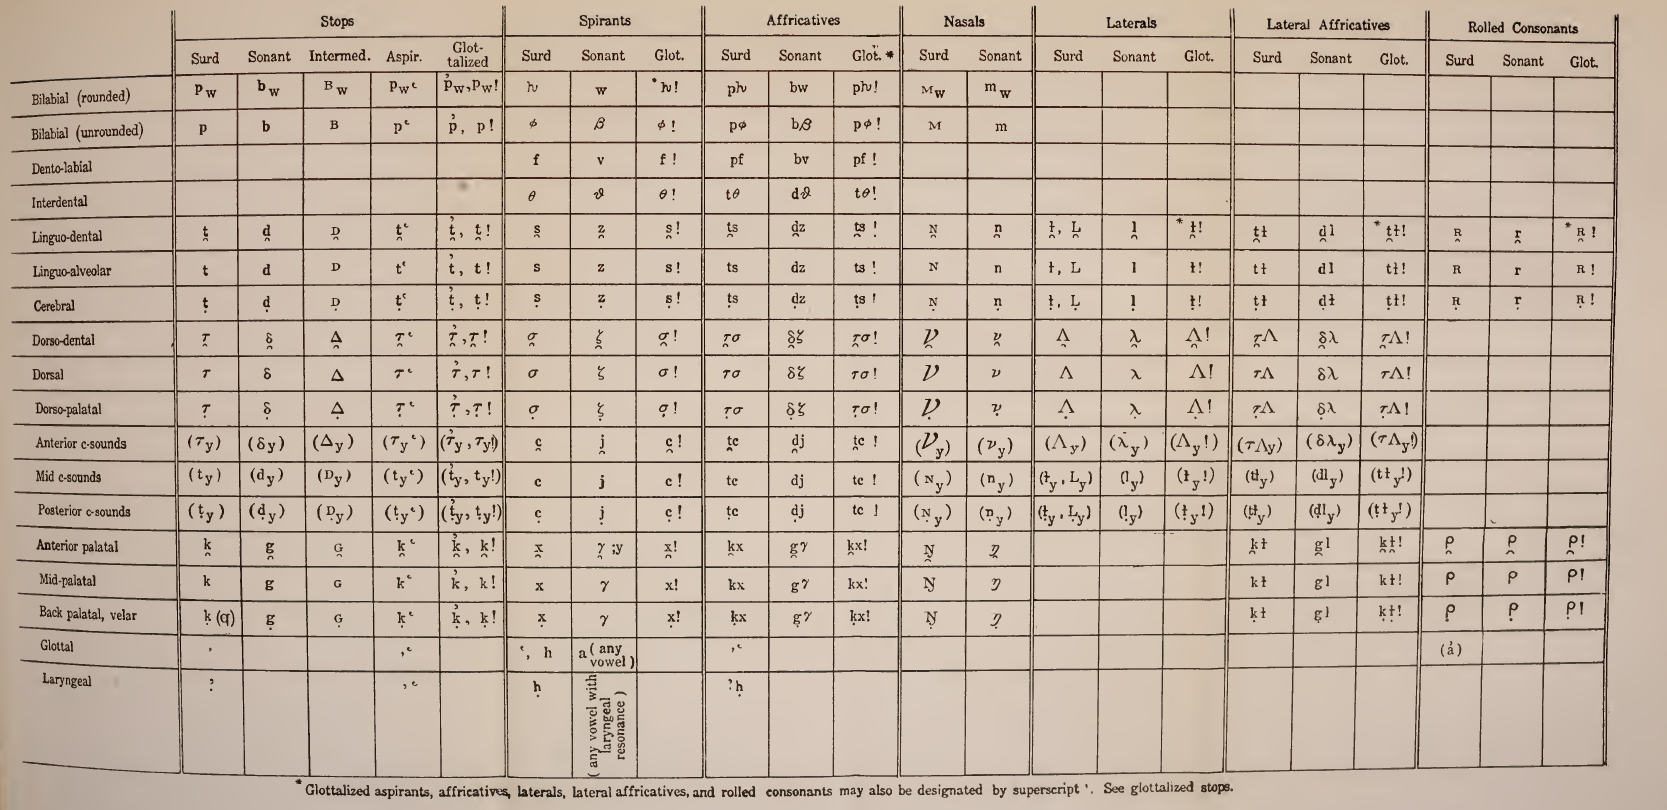
\includegraphics[width=1\linewidth]{jipa/images/americanistChart}
	\caption[Original chart of the Americanist Transcription System \parencite{boasPhoneticTranscriptionIndian1916}]{The original chart of the Americanist Transcription System \parencite[21--22]{boasPhoneticTranscriptionIndian1916} is not included in the original article. Rhotics are under the category ‘Rolled Consonants’. The small capitalized \textsc{d} is found among the ‘Stops’ category.}
	\label{fig:americanistchart}
\end{figure}


The ATS used the term ‘intermediate stop consonants’, that might be interpreted as taps, using the (small) capital grapheme D to represent them (the lower case d being reserved for the voiced apical stop).\footnote{A symbol for the flap ř exists as well. The tap and the flap were never intended to be contrasted by means of two symbols. While \textcite[88]{chomskyCurrentIssuesLinguistic1964} uses the symbol D for the tap (same as the symbol found in the original ATS but with a capital letter instead of a small capital), the flap ř might come from \textcite{smalleyManualArticulatoryPhonetics1963} who used it in opposition with the trill.}
Notably, the tap is considered as an allophone of plosives /t d/, and is not represented by an \textit{r}–based segment like in the Europeanist tradition. In the latter,  the symbol \textit{ɾ} is found to represent at the same time taps as allophones of rhotics and as allophones of plosives. In 1949, the Europeanist tradition, in its \textit{Principles of the International Phonetic Association being a description of the International Phonetic Alphabet and the manner of using it, illustrated by texts in 51 languages} \parencite{ipaPrinciplesInternationalPhonetic1949} notes for \textit{r}:

\begin{displayquote}
\textit{r}. Rolled \textit{r} as in Scottish English, Italian, Spanish, Russian. The letter is also used whenever possible to denote flapped \textit{r} (\textit{ɾ}), fricative \textit{r} (\textit{ɹ}) [sic], lingual fricationless continuant \textit{r} (\textit{ɹ}) , uvular rolled \textit{r} (\textit{ʀ}), uvular fricative \textit{r} (\textit{ʁ}) [sic] or the uvular frictionless continuant (\textit{ʁ}). \parencite[Section 26]{ipaPrinciplesInternationalPhonetic1949}
\end{displayquote}

There are also some clarification notes:

\begin{displayquote}
(d) The letter \textit{ʀ} may denote the fully rolled sound with two or more flaps of the uvula or the single–flap sound. In a language containing the two sounds as separate phonemes, the notation \textit{ʀʀ} is recommended for the fully rolled sound.

(e) The letter \textit{r} may, when convenient, replace \textit{ɹ}, \textit{ʀ} or \textit{ʁ} in the transcription of a language containing one of these three sounds but not a rolled lingual \textit{r}.

(f) The flapped sound \textit{ɾ} can generally be represented by \textit{r}. In a language such as Spanish, where a single flap and the fully rolled sound occur as separate phonemes, the notation \textit{rr} is recommended for the fully rolled sound. \parencite[Section 27]{ipaPrinciplesInternationalPhonetic1949}
\end{displayquote}

Thus, the symbol \textit{r} can be used to represent no less than 7 different phones with different manners and places of articulation (diacritics were not yet a norm at that time, so as to represent a  more open fricative or approximant, with the fricative \textit{ɹ} being next to \textit{θ} and \textit{ð}, and \textit{s} and \textit{z} in the 1949 table). The convention to duplicate the symbol does not seem clearly specified, but is left to the authors' interpretation. The use of a single symbol for these phones may be based on the idea that these sounds really belong to a single phonological class, called rhotics, which has been widely used in the literature \parencite{barryAnotherRtickle1997,scobbieVariable2006,magnusonStoryTwoVocal2007,chabotWhatWrongBeing2019} but without reaching a universal and consensual definition. While reflecting a certain theoretical stance, this ‘homonymy’ can lead to misunderstandings and to a potential bias favoring the interpretation of trill (or rolled) \textit{r} as the typical and most common phoneme represented by symbol \textit{r} despite a more nuanced situation.\\

The 1999 edition of the \textit{Handbook of the International Phonetic Association: A Guide to the Use of the International Phonetic Alphabet} \parencite{ipaHandbookInternationalPhonetic1999} says:

\begin{displayquote}
Trills are sounds like [r] is Spanish perro ‘dog’ in which the air is repeatedly interrupted by an articulator (in this case the tongue tip) vibrating in an airstream. A very short contact, similar in duration to one cycle of the vibration of a trill, is called a tap, such as the [ɾ] in Spanish pero ‘but’. \parencite[8]{ipaHandbookInternationalPhonetic1999}
\end{displayquote}
\begin{displayquote}
Note: most forms of English, French, German, Swedish do not have trills except in over–articulated speech, for instance when trying to be clear over a poor telephone line. \parencite[19]{ipaHandbookInternationalPhonetic1999}
\end{displayquote}
In this edition, there is no explicit guideline on using \textit{r} as a generic symbol to denote different phones, but there is no indication to avoid this practice, either.\\

In conclusion, the IPA mandates a generic use of the \textit{r} symbol that blurs what was actually analyzed: while it conveys the broad idea that this is a rhotic, it is left to the author(s) to somehow clarify the place(s) and manner(s) used. This imprecision, unfortunately, can be quite misleading for typological, comparative work, especially when large databases and quantitative methods are used (but even more focused, manual comparisons might be affected as well).

\subsection{‘Trills’ and ‘taps’}\label{subsec:trill_tap}

The phone alveolar trill is usually described in terms of articulation, acoustics and aerodynamics, and most of the authors refer to Spanish (or other Romance languages such as Catalan; Recasens \parencite*{recasensProductionCharacteristicsApicoalveolar1991}) for its characterization. In \textit{the Handbook of the International Phonetic Association} \parencite{ipaHandbookInternationalPhonetic1999}, the trill is described articulatorily, and the tap is described as similar to the trill but with one cycle only (using Spanish as reference) \parencite{ipaHandbookInternationalPhonetic1999}.\footnote{Please note that we do not make here a distinction between alveolar tap (‘a tap is a sound in which a brief contact between the articulators made by moving the active articulator directly towards the roof of the mouth’ \parencite[231]{ladefogedSoundsWorldLanguages1996}) and flap (‘a flap is a sound in which a brief contact between the articulators made by moving the active articulator tangentially to the site of the contact, so that it strikes the upper surface of the vocal tract in passing’ \parencite[231]{ladefogedSoundsWorldLanguages1996}), and we assume that both terms refer to the same sound. While this is clearly a simplification \parencite{derrickIndividualVariationEnglish2011}, it should not have any substantial consequences for our purposes here.}
One can wonder whether trills are produced in the same way across all languages that use them, and not just in those Romance examples. While not explicitly addressed, we may expect that [r] should refer to roughly the same speech sound in languages across the world.

On the phonemic level, it is cross–linguistically infrequent to find contrasts between two trills with different places of articulation \parencite{ladefogedLateralsTrills1977,maddiesonPatternsSounds1984}, but some languages, such as Russian \parencite{yanushevskayaRussian2015} and Toda \parencite{spajicTrillsToda1996}, are reported to contrast between an alveolar trill without secondary articulation and a palatalized alveolar trill. From an articulatory point of view, ‘trills can be produced with any of the three mobile articulators: the lips, the tongue, the uvula [...]’ \parencite[49]{ladefogedLateralsTrills1977}, but only the last two are usually considered to belong to the rhotic class, as \textit{r}–like segments, written with a <r> in the Latin–based alphabet. The lingual trill can be laminal or apical: for example, in the Illustrations of the IPA, laminal trills (also called fricative trills in Illustrations) can be found in Mbarrumbathama \parencite{verstraeteMbarrumbathamaLamalama2019} and in Czech \parencite{dankovicovaCzech1997, simackovaCzechSpokenBohemia2012}. Apical trills are found, for example, in Spanish, and are generally assumed to be the prototypical trills; they can be linguolabial, dental, alveolar or postalveolar, but linguists, in general, only consider the dental and the alveolar places \parencite{ladefogedLateralsTrills1977}. Solé’s studies \parencite*{solePhonologicalUniversalsTrilling1998,soleAerodynamicCharacteristicsTrills2002} of the aerodynamics of the trilling action made with the tip of the tongue in Spanish suggest that the initiation phase is critical:

\begin{displayquote}
The conditions for initiating lingual trilling involve (i) muscle contraction of the tongue to assume the position, shape and elasticity requirements and (ii) a sufficient pressure difference across the lingual constriction. Once trilling is initiated, tongue–tip vibration is maintained as a self–sustaining vibratory system. Articulatorily, trills exhibit more predorsum retraction than taps, thus leaving more room for the vertical movements of the tongue tip and blade, and more retracted alveolar closure. In addition, the tongue body is more highly constrained for the trill than for the tap and the former articulates less with neighboring vowels. \parencite[404]{solePhonologicalUniversalsTrilling1998}
\end{displayquote}

Two parts of the tongue are involved in the alveolar trill: the tip of the tongue, and the root of the tongue. Phonetic trills are produced with the tongue body more constrained and the predorsum more lowered than for taps \parencite{recasensStudyLightDAC1999}. The predorsum retraction leading to a pharyngeal constriction may be a characteristic of some rhotic segments including at least the trill \parencite{boyceAcquiringRhoticityLanguages2016} and could explain the late acquisition of trills observed crosslinguistically \parencite{mcleodChildrenConsonantAcquisition2018}.\\

Phonemic trills are no exceptions when it comes to allophony. Solé \parencite*[412]{solePhonologicalUniversalsTrilling1998} notes that in Spanish, taps, approximants and fricatives occur as allophones, and there is variation between dialects \parencite{pennyVariationChangeSpanish2000}. Variation in production is found in other well described languages. \textcite{rennickeVariationChangeRhotics2015} observes that in Brazilian Portuguese (which contrasts two rhotics), the rhotic allophonic family can be very large, as judged from productions ([r r̥ ɾ ɾ̥ ɾ̞ ɾ̞̥ ɹ j ɻ w ə ɚʰ ɹʰ jʰ ɻʰ ʀ ʁ χ ɦ h]); based on the Figure 8.1, p.239). \textcite{sebregtsSociophoneticsPhonologyDutch2014} for Dutch reports twenty possible variants and highlights the fact that taps that are highly frequent are not ‘failed trills or even successful trills with a single contact’ but intended as such. He favors the hypothesis that taps might historically originate from trills without excluding the possibility of a ‘reverse directionality’ \parencite[179]{sebregtsSociophoneticsPhonologyDutch2014}. The articulatory reduction and the reinterpretation of the allophonic alveolar trill can result in the emergence of allophones; for example, the change of place of articulation from alveolar to uvular, or the emergence of fricatives as ‘“failing” trills’ \parencite[412--413]{solePhonologicalUniversalsTrilling1998}. The interactions and relationships between different variants of the same phoneme /r/ are also studied (for example, for Greek \parencite{baltazaniManyFaces2013}, for Dutch \parencite{sebregtsSociophoneticsPhonologyDutch2014}, or for South–Tyrol Italian \parencite{spreaficoSociophoneticsBozenModelling2016}) in an attempt to understand the linguistic and social factors that may play a role in the variation found on the surface, and the place of the trill [r] in this allophone network.\\

Some authors suggest that, from an acoustic point of view (which is, to state the obvious, not necessarily the same as an articulatory point of view), a trill is basically a sequence (or series) of taps and, conversely, that a tap is a trill with a single period \parencite{lindauStory1985,ladefogedSoundsWorldLanguages1996}. However, there does not seem to be a consensus on the number of periods that an allophonic trill should have, varying from 2–3 closures up to 6–8, and it may depend not only on the variety, but also on the context and the speaker \parencite{henriksenAcousticCharacterizationPhonemic2010}. Moreover, the aforementioned references suggest that in a linguistic system one can observe a coexistence of a single-closure allophonic trill with a genuine tap, leading to another source of confusion. The phonetic alphabet does not capture these fine differences in the number of closures in part because there are no conventions on how to represent them.\\

One can note several conditioning factors that affect the distribution of the allophones mentioned above. The most important are probably the phonetic/ phonological environment and the broader context (i.e. the discourse settings and the communicative intentions). The phonetic and phonological environment includes the position within the syllable and the word, with intervocalic and final position favoring taps, while word– and syllable–initial positions favoring trills; trills are also more frequent in stressed syllables \parencite{eadesGayo2006,iskarousInteractionContrastProsody2010,mooneyBearnaisGascon2014}. There is indeed an association between stress and the increase in subglottal pressure \parencite{liebermanIntonationPerceptionLanguage1966}, with a minimum difference of 2 to 3 cm H$_2$O for voiced trills across the glottis \parencite{soleAerodynamicCharacteristicsTrills2002}. The wider context most frequently refers to careful or emphatic speech, and to the use of citation forms, all favoring the production of trills \parencite{breenCentralArrernte2005,bakerDariAfghanPersian2016}. Inter–speaker variation in the production of allophonic trills and taps is also somehow overlooked despite being widely accepted: ‘[...] taps are not produced in the same way in different languages nor are they always produced in the same way by different speakers of the same language’ \parencite[161]{lindauStory1985}. This ambiguous recognition status is probably related to a lack of studies addressing this type of variation. When considering the phonemic trill, an additional (sociolinguistic) source of inter–speaker variation is that individuals that fail to master the trill in languages that normatively use it, are usually considered as having a speech disorder \parencite{romano2013preliminary}, and may undergo speech therapy. Such individuals may systematically use sounds that are similar to the target trill but might be easier to articulate (e.g., alveolar approximants), but these substitution patterns seem to differ across languages and speakers (e.g., the allophonic palatal approximant [j] studied in \textcite{alfwaressRelationshipVocalTract2015} for native Arabic speakers).

\subsection{The cross–linguistic occurrence of ‘trills’}

Due to multiple reasons, which we detail below, we concur with Lindau’s \parencite*{lindauStory1985} assessment that:

\begin{displayquote}
An actual trill realization of an /r/ is not as common as might be expected from descriptions of languages, where an /r/ is often labeled as a ‘trill’. Even in languages where a possible realization is a trill, not all the speakers use a trill, and the speakers that do, have a tap and approximant allophones as well as the trill. \parencite[161]{lindauStory1985}
\end{displayquote}

In fact, the orthography used by the IPA – based on the Latin alphabet extended with additional symbols – probably had a huge impact: some symbols from the extended set might appear ‘stranger’ than others, encouraging the preponderant use of the ‘basic’ Latin IPA characters. It seems that some authors may have a preference towards the use of the symbol \textit{r} even if the actual sound is realized with one closure only, while others use the same symbol to report all ‘\textit{r}–like’ sounds (\textit{r} in some cases referring to speech sounds made at the uvular place of articulation). The historical development of the IPA itself may have contributed to this situation, as there was no symbol for the tap before 1908, with \textit{ɹ} being used for the ‘untrilled lingual \textit{r}’ (the alveolar approximant). Even after its proposal in 1908, the symbol \textit{ɾ} had to wait until 1928 before appearing in Le Maître Phonétique in the IPA chart included in reprinted Daniel Jones' article \textit{Das System der Association Phonétique Internationale (Weltlautschriftverein)} \parencite*{jonesSystemAssociationPhonetique1928}.\\

\begin{figure}
	\centering
	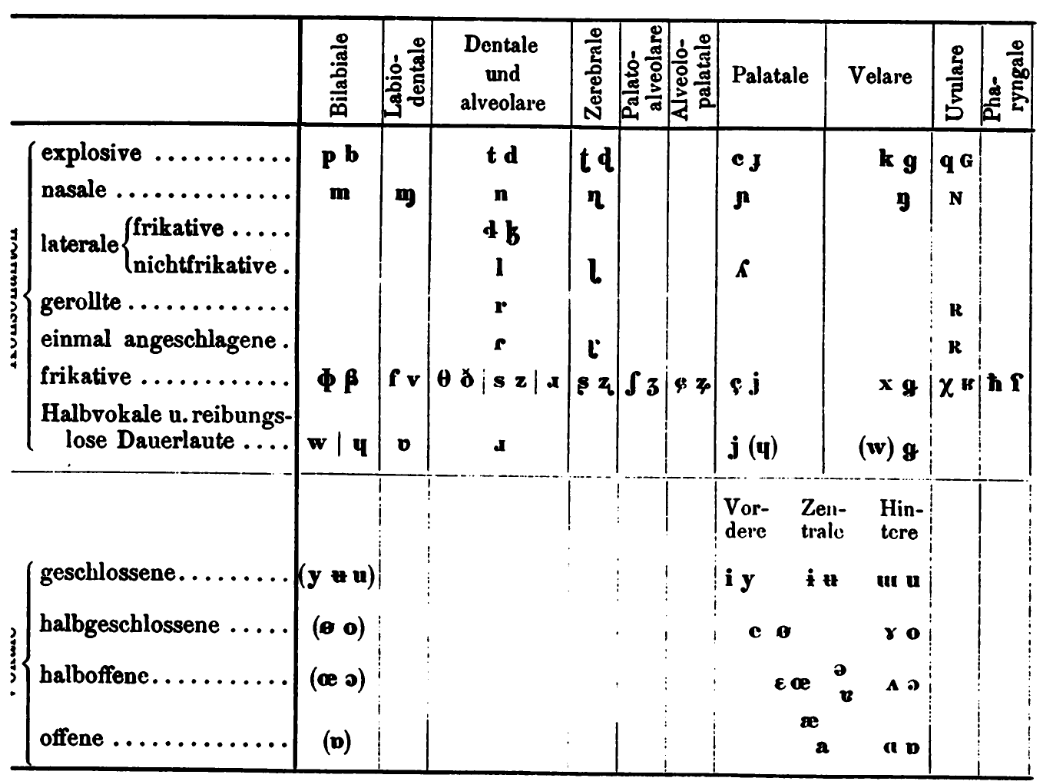
\includegraphics[width=1\linewidth]{jipa/images/jones_table}
	\caption[Chart of consonants in German of the International Phonetic Association by \parencite{jonesSystemAssociationPhonetique1928}]{The chart of consonants in German of the International Phonetic Association by \parencite[23]{jonesSystemAssociationPhonetique1928}. It is not included in the original article. ‘gerollte’ can be translated by ‘rolled’ and ‘einmal angeschlagene’ by ‘once struck’.}
	\label{fig:jonestable}
\end{figure}

While in some languages, such as Spanish and Catalan, the presence of phonemic trills and taps has been intensely studied, for many others this is still not the case. This is further complicated by contextual, dialectal, sociolectal and idiolectal variation, as well as by language contact and ‘rarity’: for example, in Bearnais (Gascon), a standard French [ʁ] might be produced as an allophone of the apical rhotics /r/ and /ɾ/  \parencite{mooneyBearnaisGascon2014}; and in Isthmus (Juchitán) Zapotec, an alveolar trill is present in ‘less than a half dozen words’ \parencite[366]{pickettIsthmusJuchitanZapotec2010}. In some language varieties, an alveolar trill allophone of the phonemic rhotic may be stigmatized (as in, for example, Japanese \parencite{labrunePhonologyJapanese2012,ooigawaPerceptionItalianLiquids2015,vanceSoundsJapanese2008} and French  \parencite{prematRouleFrancaisDans2018}. The allophonic tap can also be a source of stigmatization as in Cagliari Sardinian where it is an ‘stigmatized’ allophone of the alveolar plosives but not for the intervocalic /r/ \parencite{mereuCagliariSardinian2019}. Scottish English is a good illustration of the discrepancy between reality and a metalinguistic representation biased in favor of trills: it turns out that trills are not common in Scottish English. \textcite[57]{lawsonSocioArticulatoryStudyScottish2014} report that ‘many speakers, when questioned, will say that a typical Scottish /r/ is a trilled /r/, even though this is rarely the case nowadays’, and many recent studies systematically show the rarity of trilling in Scottish English \parencite{pukliInvestigationSociophonetiqueAnglais2006,stuart-smithDerhoticisationScottishEnglish2014,jauriberryRhotiquesRhoticiteEcosse2016}. The large variation observed in the phonemic trill may be in part explained by the fact that allophonic trills are articulatorily more complex than allophonic taps (the latter being acquired earlier than the former, \parencite{mcleodChildrenConsonantAcquisition2018}), require more energy and a precise control of the parameters involved in its aerodynamics, which can lead to trilling failure.\\

Therefore, it seems that more than a century after the publications of the first international guidelines on phonetic transcription, the way the symbol \textit{r} is used throughout the linguistic community is still not consistent and universally shared. We argue here that this situation is highly detrimental and significantly hinders the capacity to develop a typology of the [r] sound and of the rhotics from a phonetic perspective. Answering questions such as whether or not [r] is rare becomes unnecessarily complicated, and querying databases needs extra care to identify and control for the noise induced by the (sometimes implicit) use of different guidelines and expectations concerning the way sounds should be represented.

\section{Data and methods}

To address the problem with the generic use of \textit{r}, we conducted a full analysis of all the articles published in the peer–reviewed \textit{Journal of the International Phonetic Association} in the collection \textit{Illustrations of the IPA}.\footnote{ISSN: 0025–1003 for the printed, and 1475–3502 for the \href{https://www.cambridge.org/core/journals/journal-of-the-international-phonetic-association}{online editions}}
The journal began at the end of the 19th century, initially titled \textit{Le Maître Phonétique} and fully written in the \textit{Alphabet Phonétique International} (API), or \textit{International Phonetic Alphabet} (IPA) in English, changing its name to JIPA only in 1971, and moving away from articles written in IPA (in different languages) and towards standard orthographies. The \textit{Illustrations of the IPA} section first appeared in \textit{JIPA}'s 20th volume in 1990, following a decision of the 1989 Kiel Convention \parencites[77--80]{ipaIllustrationsIPA1990,roachReport1989Kiel1989}. Since then, \textit{Illustrations} has been compiled in two volumes, in 1995 and 1999. Prior to the creation of the \textit{Illustrations} section, transcriptions of ‘The North Wind and the Sun’, dating back to the earliest days of \textit{Le Maître Phonétique}, were published variously in \textit{The Principles of the International Phonetic} Association \parencite{ipaPrinciplesInternationalPhonetic1949} and particular volumes under various sections, such as \textit{spesimɛn} (Specimen).\\

\begin{figure}
	\centering
	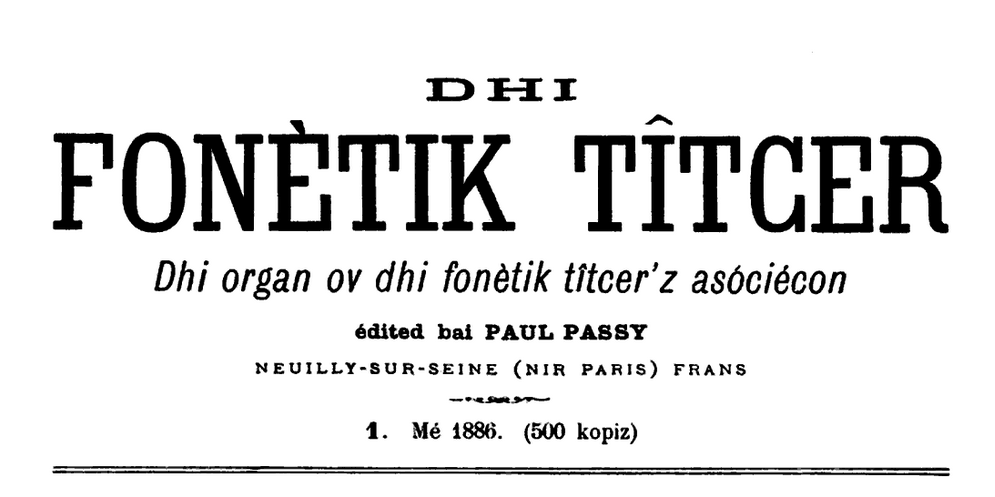
\includegraphics[width=1\linewidth]{jipa/images/phonetic_teacher}
	\caption[Illustration of the title of first issue of the journal of the association ‘lə mɛ${:}$trɘ fɔnetik’]{As the International Phonetic Association evolved \parencite{esling40thAnniversaryJIPA2010}, so did its transcription system and its journal. This title of first issue of the journal of the association ‘lə mɛ${:}$trɘ fɔnetik’ / ‘dhi fonètik tîtcer’ is not included in the original article.}
	\label{fig:phoneticteacher}
\end{figure}

The original aim of \textit{Illustrations} was to offer a linguistic foundation to the written symbols, or graphemes, chosen to represent the sounds of spoken languages, with each illustration focusing on a single variety (‘language’, dialect or sociolect). The idea was and still is that each such contribution should define the phonemic inventory (or, if not possible, at least to sketch a first version) using the IPA symbols. Some illustrations also contain a summary of the studies on the variety, and a brief sociolinguistic sketch (including speaker population size, socioeconomic status of the informants, bi–/multilingualism, and relationships to an official variety). Over the years, \textit{Illustrations} has provided invaluable insights into the sound systems of a large number of languages and varieties. \\

Each illustration provides a narrative which is, in general, based on a single speaker who pronounces the poem ‘The North Wind and the Sun’ in their own variety, but some authors chose to include a different story. This narrative is recorded and then transcribed. The most recent instructions for contributors \parencite{ipaInstructionsContributors2021} indicate that the transcription must be ‘phonemic’ (highlighting the contrasts in the language) but that a ‘narrow’ transcription can also be added (highlighting the phonetic specificities of the variety and/or of the speaker(s)’s idiolect(s)).

\subsection{Data collection}\label{subsec:data_coll}

The primary data consists of all the relevant information extracted from illustrations available on the \textit{JIPA} website. Due to a change of style after 2000, when Cambridge University took over the production of JIPA \parencite{ipaPublicationJournalInternational2000}, we split them into those published before 2000 (42 illustrations), and those published between 2000 and 2020 (168 illustrations). We checked the consistency of the pre–2000 illustrations with their re–edited version in the \textit{Handbook of the International Phonetic Alphabet: A guide to the use of the International Phonetic Alphabet} in 1999 (IPA, 1999), and we included two additional illustrations present only in this source but absent from the \textit{JIPA} website (American English by Ladefoged \parencite*[41--44]{ipaHandbookInternationalPhonetic1999} and Portuguese (European) by Cruz \parencite*[126--130]{ipaHandbookInternationalPhonetic1999}), resulting in a total of 213 illustrations, including 46 published before 2000.\\

We compiled the extracted information in a table (in CSV format, available in the Supplementary Materials accompanying the original article), with the following information:

\begin{itemize}
	\item[–] the title of the illustration (which corresponds to the name of the lect/variety),
	\item[–] the year of publication of the illustration (for those recent illustrations included in the First view section of the JIPA website \parencite[472]{arvanitiEditorialReportJIPA2019}, we used the year the illustration appeared online which does not necessarily coincide with the year of publication),
	\item[–] the author’s/authors’ name(s), affiliation(s), e–mail address(es),
	\item[–] the geographical area, the country/countries, and the specific region(s) in which the variety is spoken,
	\item[–] the size of the speaker population, if available,
	\item[–] if available, information concerning the informant(s), such as the sex, age and
	socio–economic status,
	\item[–] the section(s) of the narrative transcription which allowed us to infer if the transcription is ‘phonemic’ (i.e., using a phoneme representation, usually known as a ‘broad transcription’) or rather ‘phonetic’ (i.e., using phonetic representation, usually known as a ‘narrow transcription’) \parencite[Section 5]{ipaHandbookInternationalPhonetic1999}. While some illustrations have one transcription only, a few of them include both phonemic and phonetic transcriptions (for more details, see the \autoref{subsec:pht_phm}).
\end{itemize} 

We manually added the location where the variety is spoken, and, when there was no indication of the actual geographical coordinates, we used Google maps and Open Street maps to estimate the latitude and longitude, starting from the reported name of the place. We used a broad classification of macroareas based on that proposed by Glottolog \parencite{glottolog}.

\subsection{Defining and coding ‘\textit{r}–like’ sounds}

We decided to focus on two characters \textit{r} and \textit{ɾ} (respectively lower–case R and fish–hook R [\cite{pullum1996phonetic}]) and the characters derived from these through the addition of diacritic(s). In our analysis we refer to the lower–case R as the \textsc{trill}, and to the fish–hook R as the \textsc{tap}.\\

We looked for their presence in the consonant chart, and the transcription(s) of a narrative given at the end of the illustrations. We then considered the ‘descriptive labels’, the way authors refer to symbols, following, in most cases, the phonetic categories given to the symbols in the consonant chart found at the beginning of each illustration (place of articulation, manner of articulation and voicing). For some older illustrations no such chart is given, leading us to retrieve the labels from the indications present in the text. Our analysis is focused on the alveolar trill and the alveolar tap, leaving the other rhotics for  future studies, but we nevertheless listed the other segments mentioned in the illustrations when they can potentially be considered as ‘rhotics’ based on \textcite{magnusonStoryTwoVocal2007}‘s classification (for example \textit{ɹ}, \textit{ɻ~~}, \textit{ɽ}, \textit{ʀ}, \textit{ʁ}), to provide an overview of the rhotics and ‘\textit{r}–like’ sounds present in the illustrations and to facilitate future work. 

\subsection{Counting ‘\textit{r}–like’ sounds}

As we are mostly interested in the use of trill and tap in the transcribed narrations of Illustrations here, we  manually counted them specifically focusing on:

\begin{itemize}
	\item[–] the number n$_\textrm{[r]}$ of tokens of r in the phonetic transcription
	\item[–] the number n$_\textrm{/r/}$ of tokens of r in the phonemic transcription
	\item[–] the number n$_\textrm{[ɾ]}$ of tokens of ɾ in the phonetic transcription
	\item[–] the number n$_\textrm{/ɾ/}$ of tokens of ɾ in the phonemic transcription
	\item[–] the  number n$_\textrm{ʀ}$ of rhotic tokens: this is based on the segments we considered as rhotics in the transcriptions given by the authors. We looked for the different symbols that were used for the trill, tap, and other \textit{r}–based segments, checking what the authors wrote about whether we should consider them as rhotics or not (for example, we excluded from this count the \textit{ɾ} in phonetic transcriptions when they were an allophone of a plosive). In some cases, we looked at the orthographic transcription that was provided by the authors to give us clues about <r> segments that could be omitted or realized differently from what was expected. When several transcriptions are provided, we have used the highest number n$_\textrm{ʀ}$ across the different transcriptions.
\end{itemize} 

An additional logical variable denoting the presence or absence of <r> in the orthographic system of the language or in the transliteration was added if available. For example, in some illustrations where the language described uses a Cyrillic alphabet, we find in the transliterations <r> standing for <p>, in which case we consider that the language does contain <r> in its orthography. \\

Although this data was collected by a single coder (RA), this was done in several separate ‘rounds’, which enabled quality checking and, if necessary, correction of earlier rounds in subsequent later rounds. The first round involved the collection of metadata for the illustrations and segments of interest; the second involved the manual addition of geographic locations. The collection of quantitative data was done over two rounds, which consisted of counting \textit{r} tokens in the transcriptions, followed by counting \textit{ɾ} tokens.

\subsection{Counting all segments n$_\textrm{Seg}$}

Finally, in order to normalize the number of occurrences of rhotics across the illustrations, we also counted the total number of segments in each transcription. Although all the transcriptions come from \textit{Illustrations}, there were inconsistencies in the format in which we recovered them:

\begin{itemize}
	\item[–] some transcriptions are available in text format (.txt) from \citeauthor{bairdBlowingWindUsing2021} (in press) (available on: \href{https://github.com/SimonGreenhill/jipa}{\texttt{https://github.com/} \texttt{SimonGreenhill/jipa}})
	\item[–] when possible, transcriptions were copy–pasted from the PDF of the illustrations or from the \textit{Illustrations} web page hosted by the \textit{Journal of the IPA}
	\item[–] some transcriptions from which copy–pasting was not possible were submitted to Optical character recognition (OCR) using the R package \texttt{tesser}-\texttt{act} \parencite{ooms2019tesseract} and corrected for potential errors or were manually typed.
\end{itemize}

If there was more than one transcription in an illustration (for example, one phonemic and one phonetic transcription, or for different varieties), we counted  the number of segments in the broadest transcription available, or by averaging the counts found in the transcriptions when they had the same level of phonetic precision. We wrote an R script to automatically count the alphabetical segments, using regular expressions excluding numbers, diacritics, second manners of articulation, suprasegmental symbols and punctuation.

\subsection{Phonetic and phonemic transcriptions}\label{subsec:pht_phm}

One of the most important and tedious steps was to classify the transcriptions according to their degree of detail. For this, we decided to look specifically at the information provided by the authors, mostly in the section headers, without any interpretations or inferences of our own. Because of the great variability in the naming of the section headers, it was nevertheless necessary to harmonize them. Therefore, we defined a binary distinction between ‘phonemic’ and ‘phonetic’ transcriptions, as follows. A phonetic transcription is inferred for section headers containing the terms ‘phonetic’, ‘narrow’, ‘allophonic’, ‘semi–narrow’, and/or ‘detailed’, while a phonemic transcription corresponds to the sections containing the following terms ‘phonemic’ and/or ‘broad’. In some cases, the authors specify that their transcription was either ‘broad phonetic’ or ‘narrow phonemic’ [sic]; here, we only kept the terms ‘phonetic’ and ‘phonemic’ to characterize these transcriptions.\\

73 transcriptions were still difficult to classify due to a lack of information, in which case, by default, we made the choice to systematically consider the transcriptions phonetic. This stems from the assumption that the purpose of Illustrations is to convey the phonetic realization of the language, as it is explicitly mentioned in the report on the 1989 Kiel Convention that the transcription should represent ‘what is actually recorded on the tape rather than an idealization of what might have been uttered’ \parencite[77]{roachReport1989Kiel1989}, even if this representation may be rather broad.\footnote{We have performed another analysis on the recommendation of the associate editor (available in the Supplementary Materials of the original article). The coding aimed at comparing the symbols present in the consonant chart and those present in the narrative transcription. If some segments were present in the narrative but not in the consonant chart, then the transcription could be considered phonetic. Of the 73 transcriptions, 31 were reinterpreted as phonemic (and 42 as phonetic. Working on a case by case basis poses the problem of adding a new bias in defining what is a phonetic and phonemic transcription when in most cases it is a mixture of both with some phonological classes being more detailed than others. When focusing on illustrations that have an \textit{r} somewhere in the transcription (or in the consonant chart), we find that 46 illustrations do not specify if the transcription is phonemic or phonetic. Of these 46 illustrations, 14 transcriptions were considered phonemic and 32 were considered phonetic.} This methodological choice is furthermore coherent with an approach in which the burden of the proof is ours: apparent trills are considered as trills as long as we cannot provide any strong arguments in favor of a non–trilled interpretation. 

\section{Results}

\subsection{General results}

\subsubsection{Year of publication}

It can be seen in \autoref{fig:graphyearjipa} that the Illustrations section started to be systematically published each year in 1990, with rather sporadic occurrences before this date. In total, we collected 213 illustrations covering 51 years (from 1971 to 2021), ranging between 1 and 22 per year with an average of 5.3. There is a difference between the date of publication on the Cambridge website and the date of publication in a \textit{JIPA} issue, usually about once year (see \autoref{subsec:data_coll} for details concerning the date of appearance in FirstView vs the publication date).

\begin{figure}
	\centering
	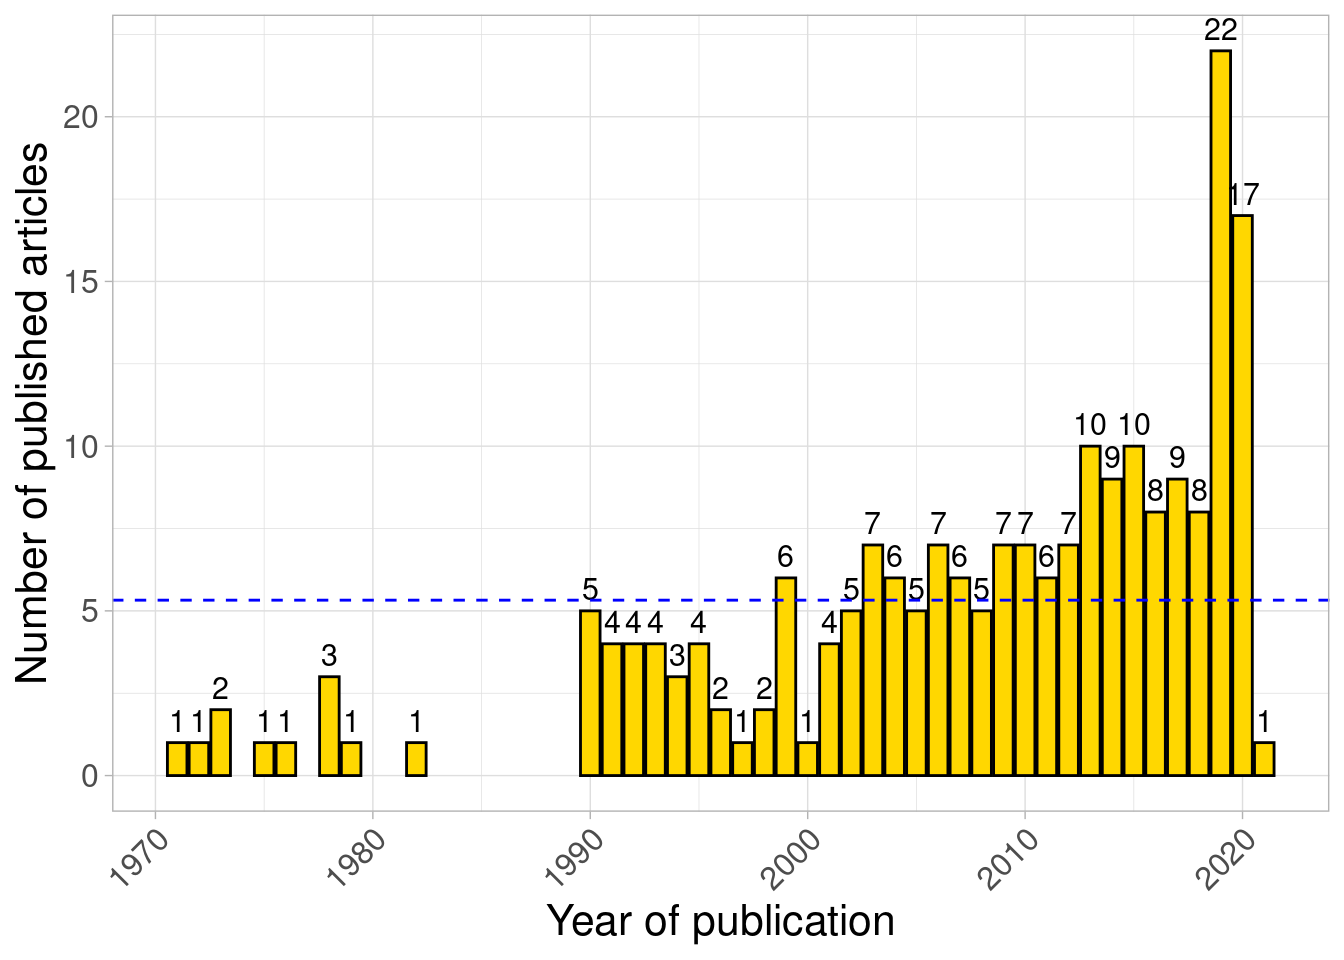
\includegraphics[width=1\linewidth]{jipa/images/graph_year_JIPA}
	\caption[Numbers of \textit{Illustrations of the IPA} publications per year]{Numbers of publications per year (yellow bars) with their average across all years (blue dashed line). Please note that some very recent illustrations might not yet be included in an official issue but only available on the journal’s website as FirstView. The figure does include First View articles with their online publication year.}
	\label{fig:graphyearjipa}
\end{figure}

\subsubsection{Informant characteristics}

For our purposes here, there might be speaker–related differences that are relevant, such as in age and gender (\autoref{fig:graphagejipa}). It is not clear if many authors are aware of any idiosyncrasies their informant(s) may have: this can be so because this is not the purpose of their illustration, or because they do not consider this as an important aspect when capturing the overall phonology/phonetics of the variety. In some cases, the authors explicitly state that they want speakers as ‘representative of the variety’ as possible \parencite[109]{namboodiripadMalayalamNamboodiriDialect2017a}.\\

Finally, since the authors are themselves academics, they tend to select speakers that are familiar with this environment, so most informants are considered as (well) educated and with a ‘correct’ pronunciation (according to the authors). Because the accessibility of the informants is an important factor, it is not uncommon for them to be students, researchers (some being the authors themselves) or teachers.

\begin{figure}
	\centering
	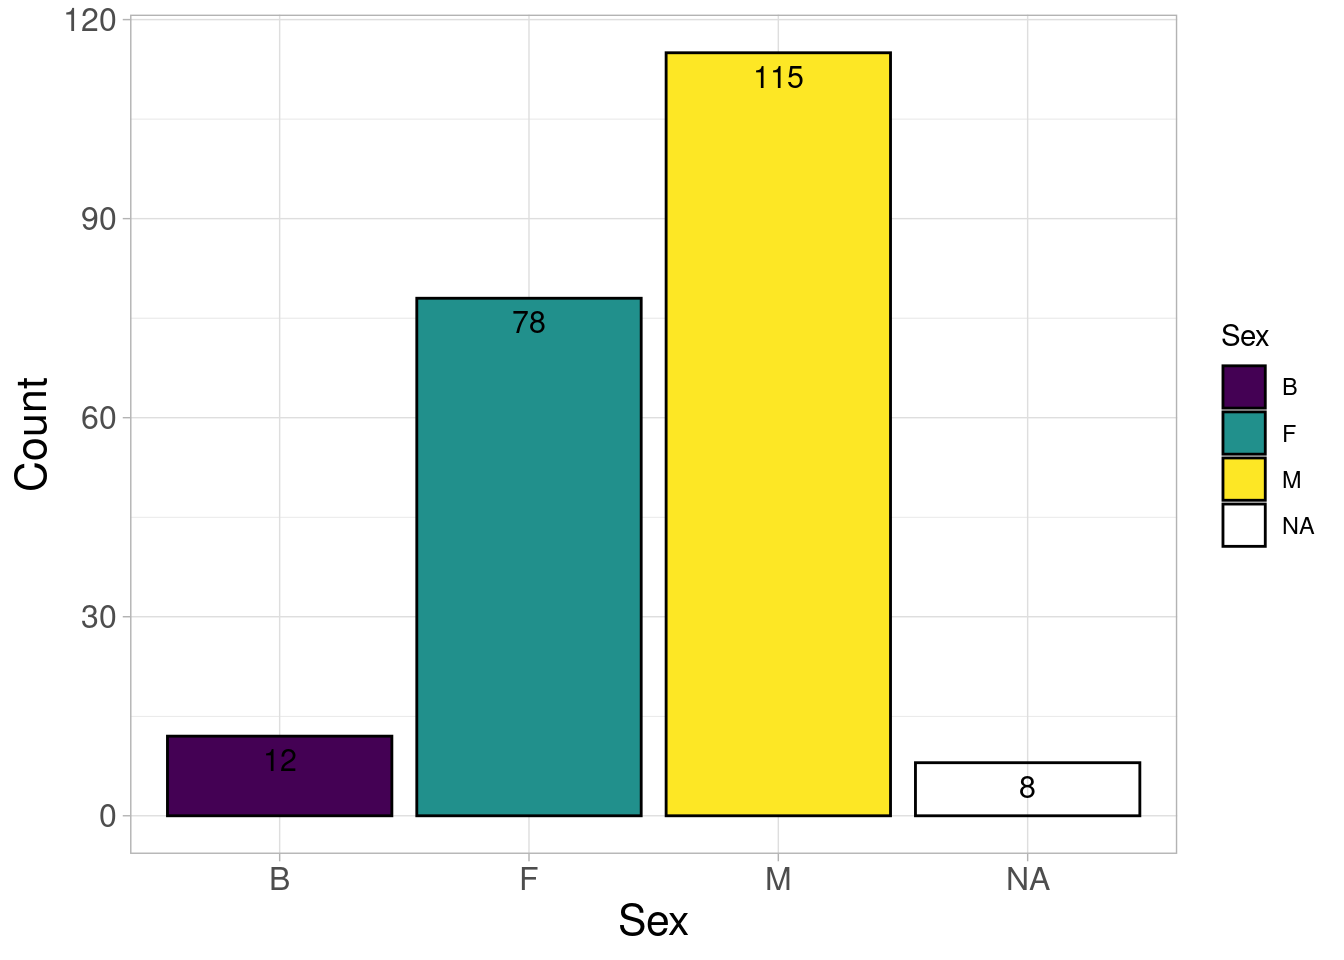
\includegraphics[width=0.475\linewidth]{jipa/images/graph_informant_JIPA}
	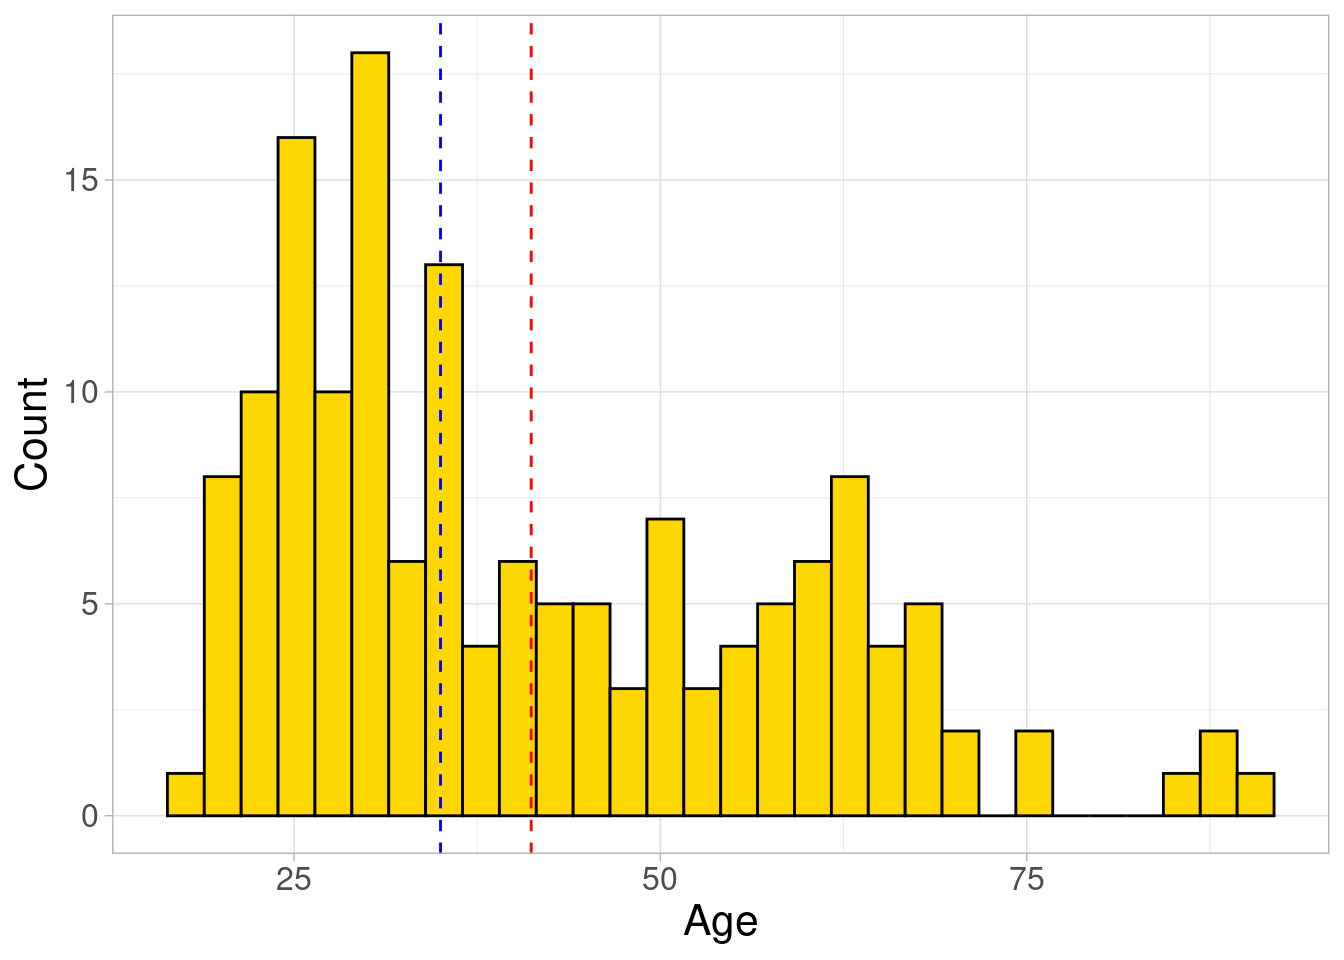
\includegraphics[width=0.475\linewidth]{jipa/images/graph_age_JIPA}
	\caption[Informant characteristics of the \textit{Illustrations of the IPA}]{Informant characteristics. Left: the distribution of informants' sex (F = female, M = male, B = both, i.e. the recording of at least 1M \& 1F used for the transcription, NA = data not communicated). Right: the distribution of the age of the informants, with mean 41 (red dashed line) and median 35 (blue dashed line).}
	\label{fig:graphagejipa}
\end{figure}


\subsubsection{Geographic distribution, families and population size}

There is an over–representation of Eurasian languages, in particular Indo–European languages, and just a few Australian languages (see Figures \ref{fig:graphfamiliesjipa} and \ref{fig:graphmacroareajipa}). Among the illustrations reviewed, a few languages are spoken by large populations and a few have very small speaker populations: the population of a variety covered by Illustrations is about 12,000,000 speakers on average, with a median of 175,000 (\autoref{fig:graphpopulationjipa}).

\begin{figure}
	\centering
	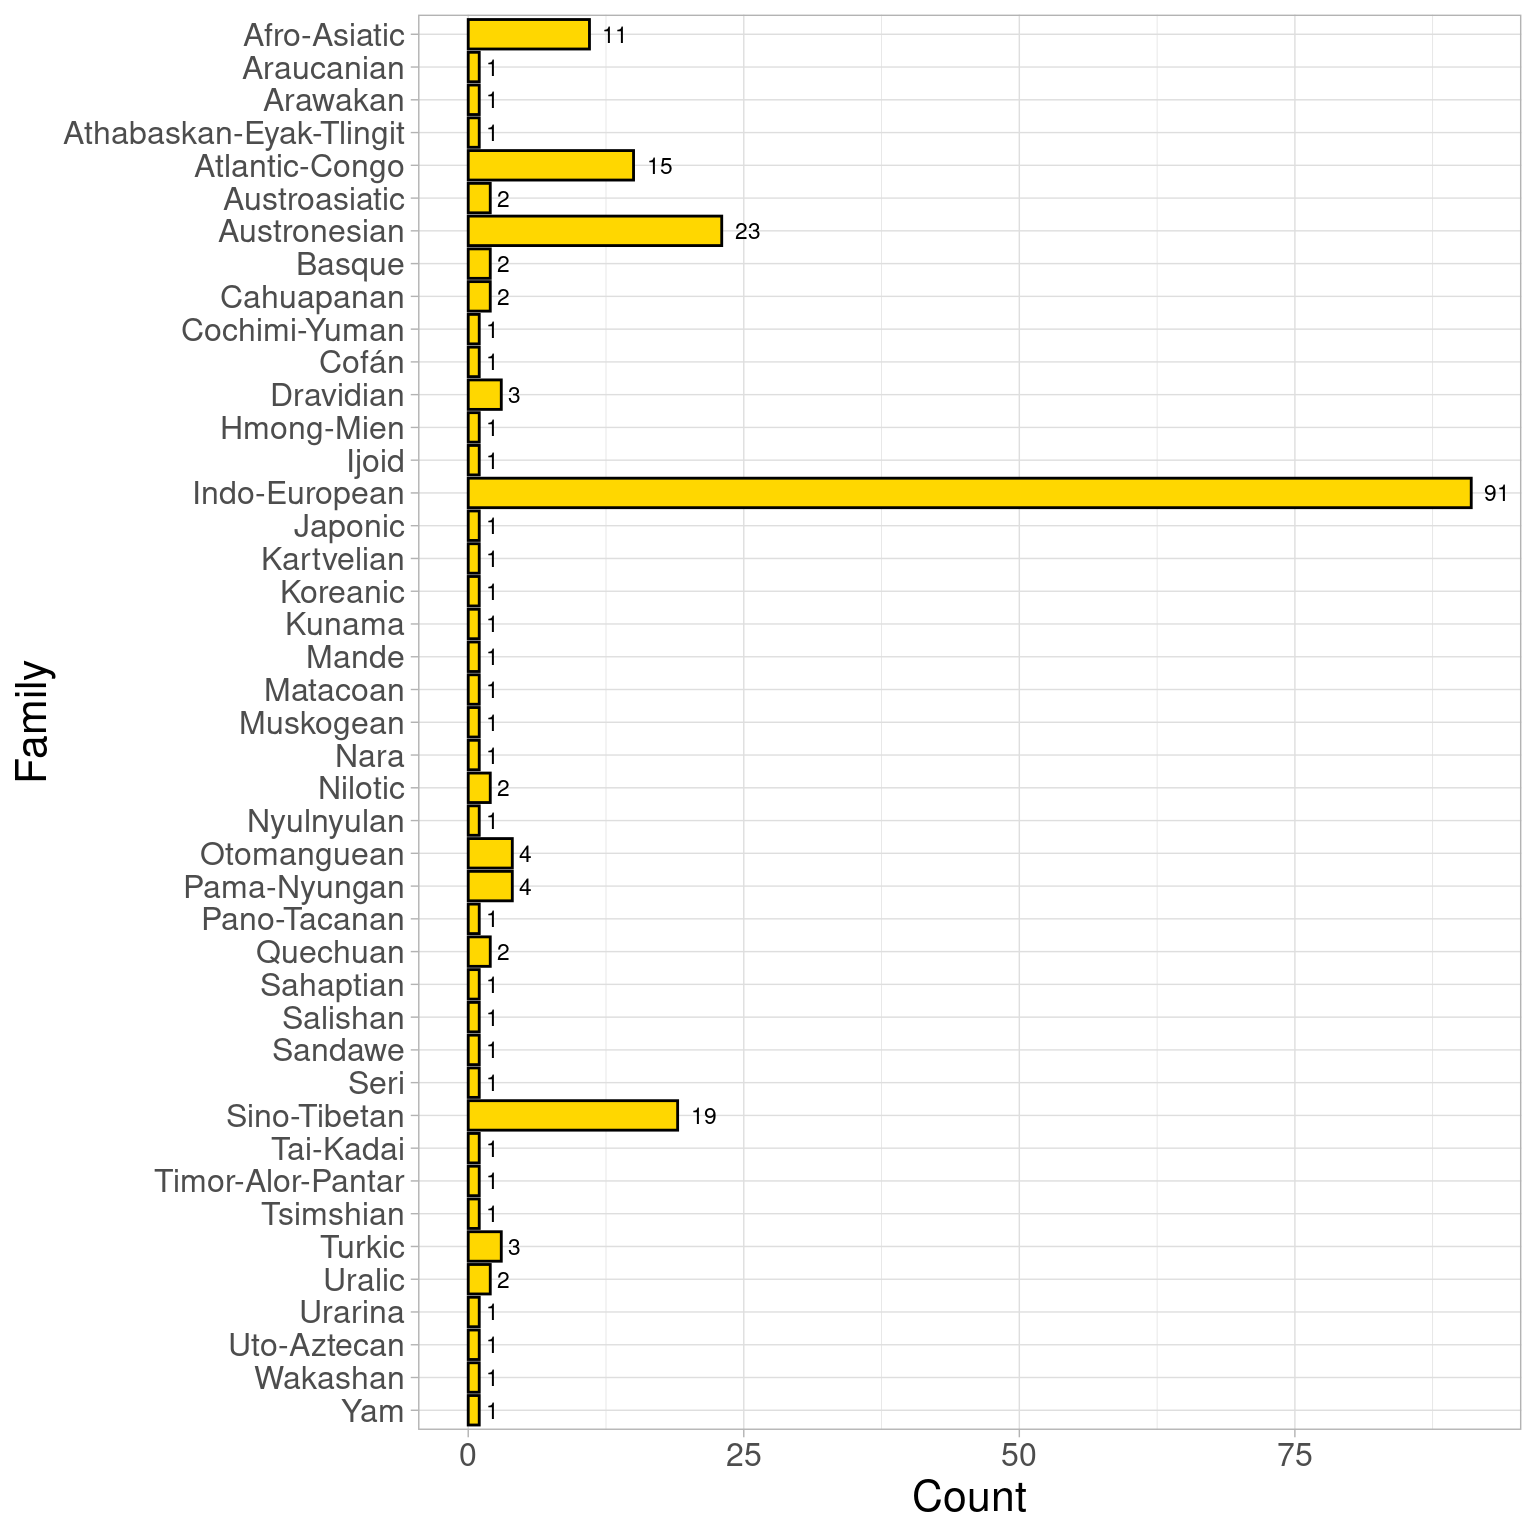
\includegraphics[width=1\linewidth]{jipa/images/graph_families_JIPA}
	\caption[Distribution of languages by family]{Distribution of languages by family based on family classifications in Glottolog \parencite{glottolog}}
	\label{fig:graphfamiliesjipa}
\end{figure}

\begin{figure}
	\centering
	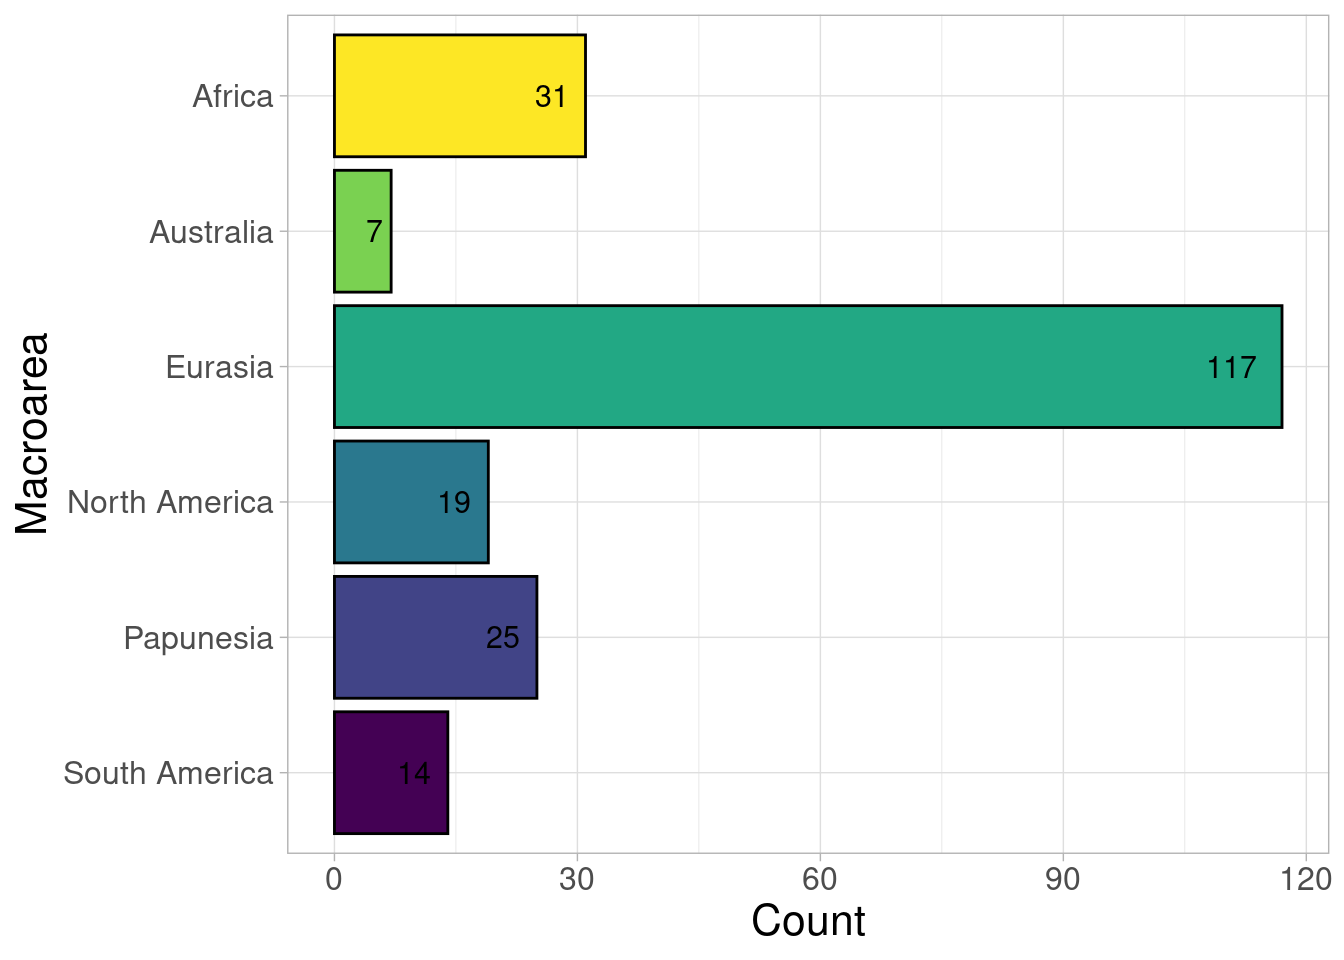
\includegraphics[width=1\linewidth]{jipa/images/graph_macroarea_JIPA}
	\caption[Distribution of languages by macroarea]{Distribution of languages by macroarea.}
	\label{fig:graphmacroareajipa}
\end{figure}

\begin{figure}
	\centering
	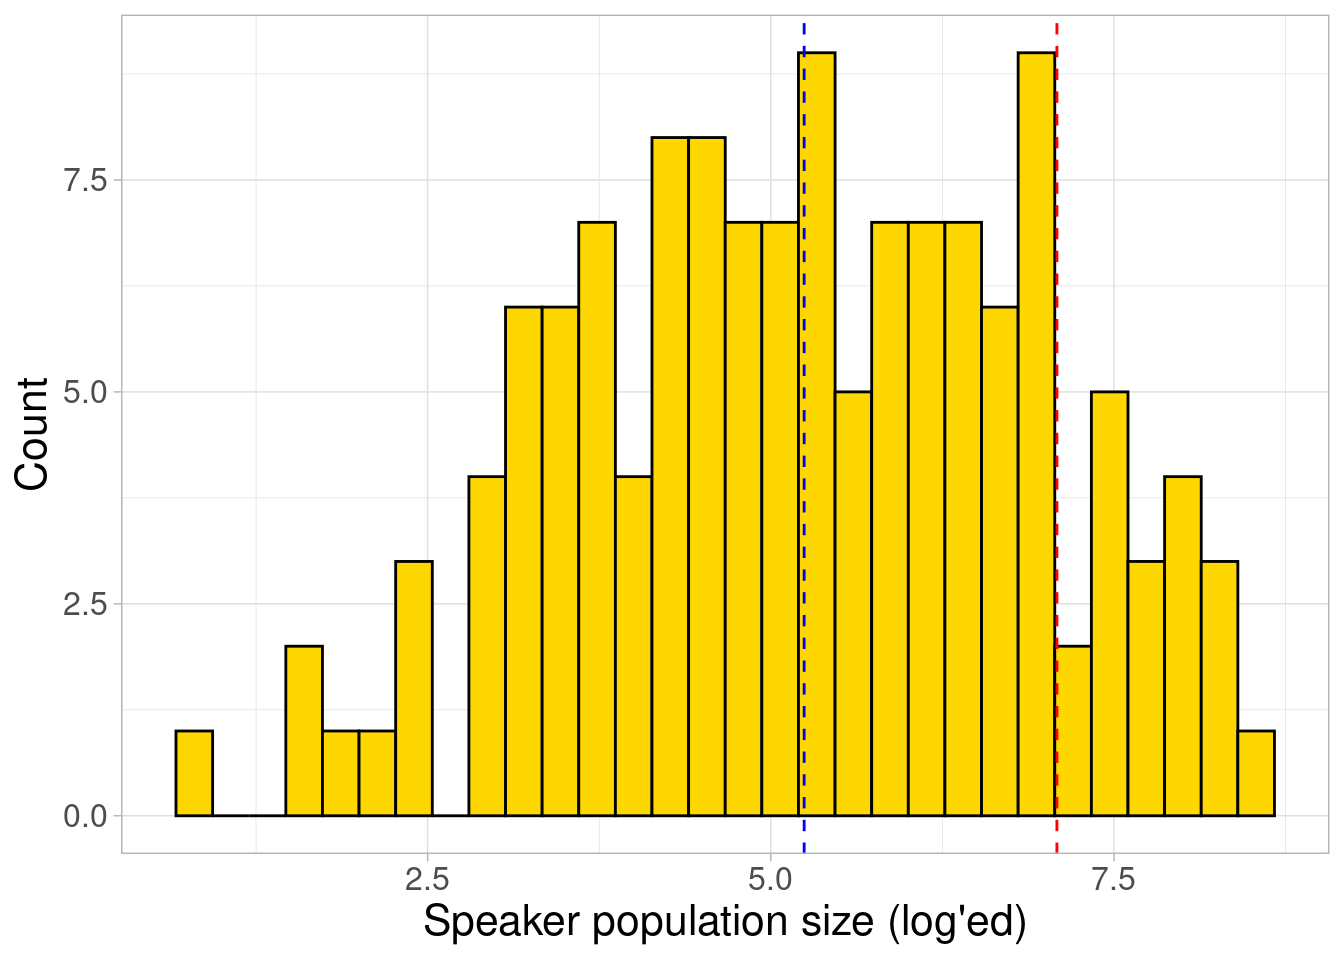
\includegraphics[width=0.7\linewidth]{jipa/images/graph_population_JIPA}
	\caption[Distribution of the log speaker population size]{The distribution of the log speaker population size, showing the mean (12,000,000 or 7.08 on the log scale; red dashed line) and the median (175,000 or 5.24 on log scale blue dashed line).}
	\label{fig:graphpopulationjipa}
\end{figure}

\subsection{Transcriptions}

\subsubsection{Phonetic and phonemic transcriptions}

Of the 213 illustrations, most had only one type of transcription (120 only had a phonetic transcription and 38 only a phonemic one) while 54 had both (phonetic and phonemic). The latter are the most informative for comparing the choice of the phonemes with their actual phonetic realizations. Finally, one single illustration did not have any transcribed narrative, this illustration corresponding to ‘Notes of a Westmeath dialect’ published in 1971 in the first volume of the \textit{Journal of the International Phonetic Alphabet}. 

\subsubsection{Orthographic transcription and transliteration}

Among the illustrations, there are several orthographic systems besides the Latin alphabet, and some of the studied languages of oral tradition do not have any orthographic system. Of the 213 illustrations, there are 134 (63\%) where we found an <r> in the orthography or in the transliteration. Among these, there are 47 (35\%) languages where a double <rr> was used (we do not exclude the possibility that other languages could also use <rr> in general, but the short length of the narrative does not allow us to provide a definite answer). There are 13 (6\%) illustrations where the language does not have an <r> in the orthography, and 66 (31\%) where either the language has no written tradition, or does not use the Latin alphabet and does not provide any transliteration in the Latin alphabet.

\subsection{‘\textit{r}–like’ sounds}

\subsubsection{\textit{r} in transcriptions}

We focus on the illustrations where the symbol \textit{r} is present: there are 136 illustrations (64\%) where \textit{r} is present in the consonant chart (105 illustrations) or there is at least an [r] or an /r/ in one of the narrative transcriptions (31 illustrations). The analyses presented in the rest of the article are based on this corpus. Among the 105 illustrations of the first type, 84 associated \textit{r} with the ‘trill’ or ‘rolled’ manner of articulation, based on the descriptive label derived from the consonant chart. In 16 cases, the usage of \textit{r} does not match with an actual trill description. An overview of the consonant charts leads us to consider that the \textit{r} is used for several manners of articulation (as an ‘approximant’, ‘tap or flap’, ‘plain tap’, ‘flap’, ‘fricative or approximant’), different places of articulation (ranging from ‘dental’ to ‘velar’), or sometimes is only just (under)specified as a ‘rhotic’. As an example, in the Shipibo illustration \parencite[282]{valenzuelaShipibo2001} it is stated that ‘[t]he symbol /r/, chosen for its simplicity, also represents a highly variable segment’. There are also 5 cases where there is no descriptive label that can be derived from the consonant chart or the illustration, preventing us from inferring what r stands for. We did not change the symbols when the \textit{r} did not match with an actual trill description.

We therefore divide the illustrations in three categories according to the type of transcription they include, and we present below the results per category, starting with the more informative with regard to phonetic substance.

\paragraph{Illustrations with both phonemic and phonetic transcriptions}

The first category includes 37 illustrations where the authors provide both phonemic and phonetic transcriptions, and which include at least one occurrence of an \textit{r} either in one of the transcriptions or in the consonant chart. Having both these transcriptions allows us to compare the phonemic transcription (which is the result of the linguistic analysis of which contrasts are important in the language) and the phonetic transcription (which arguably should be closer to the phonetic reality of what the speakers actually produced).

\begin{figure}
	\centering
	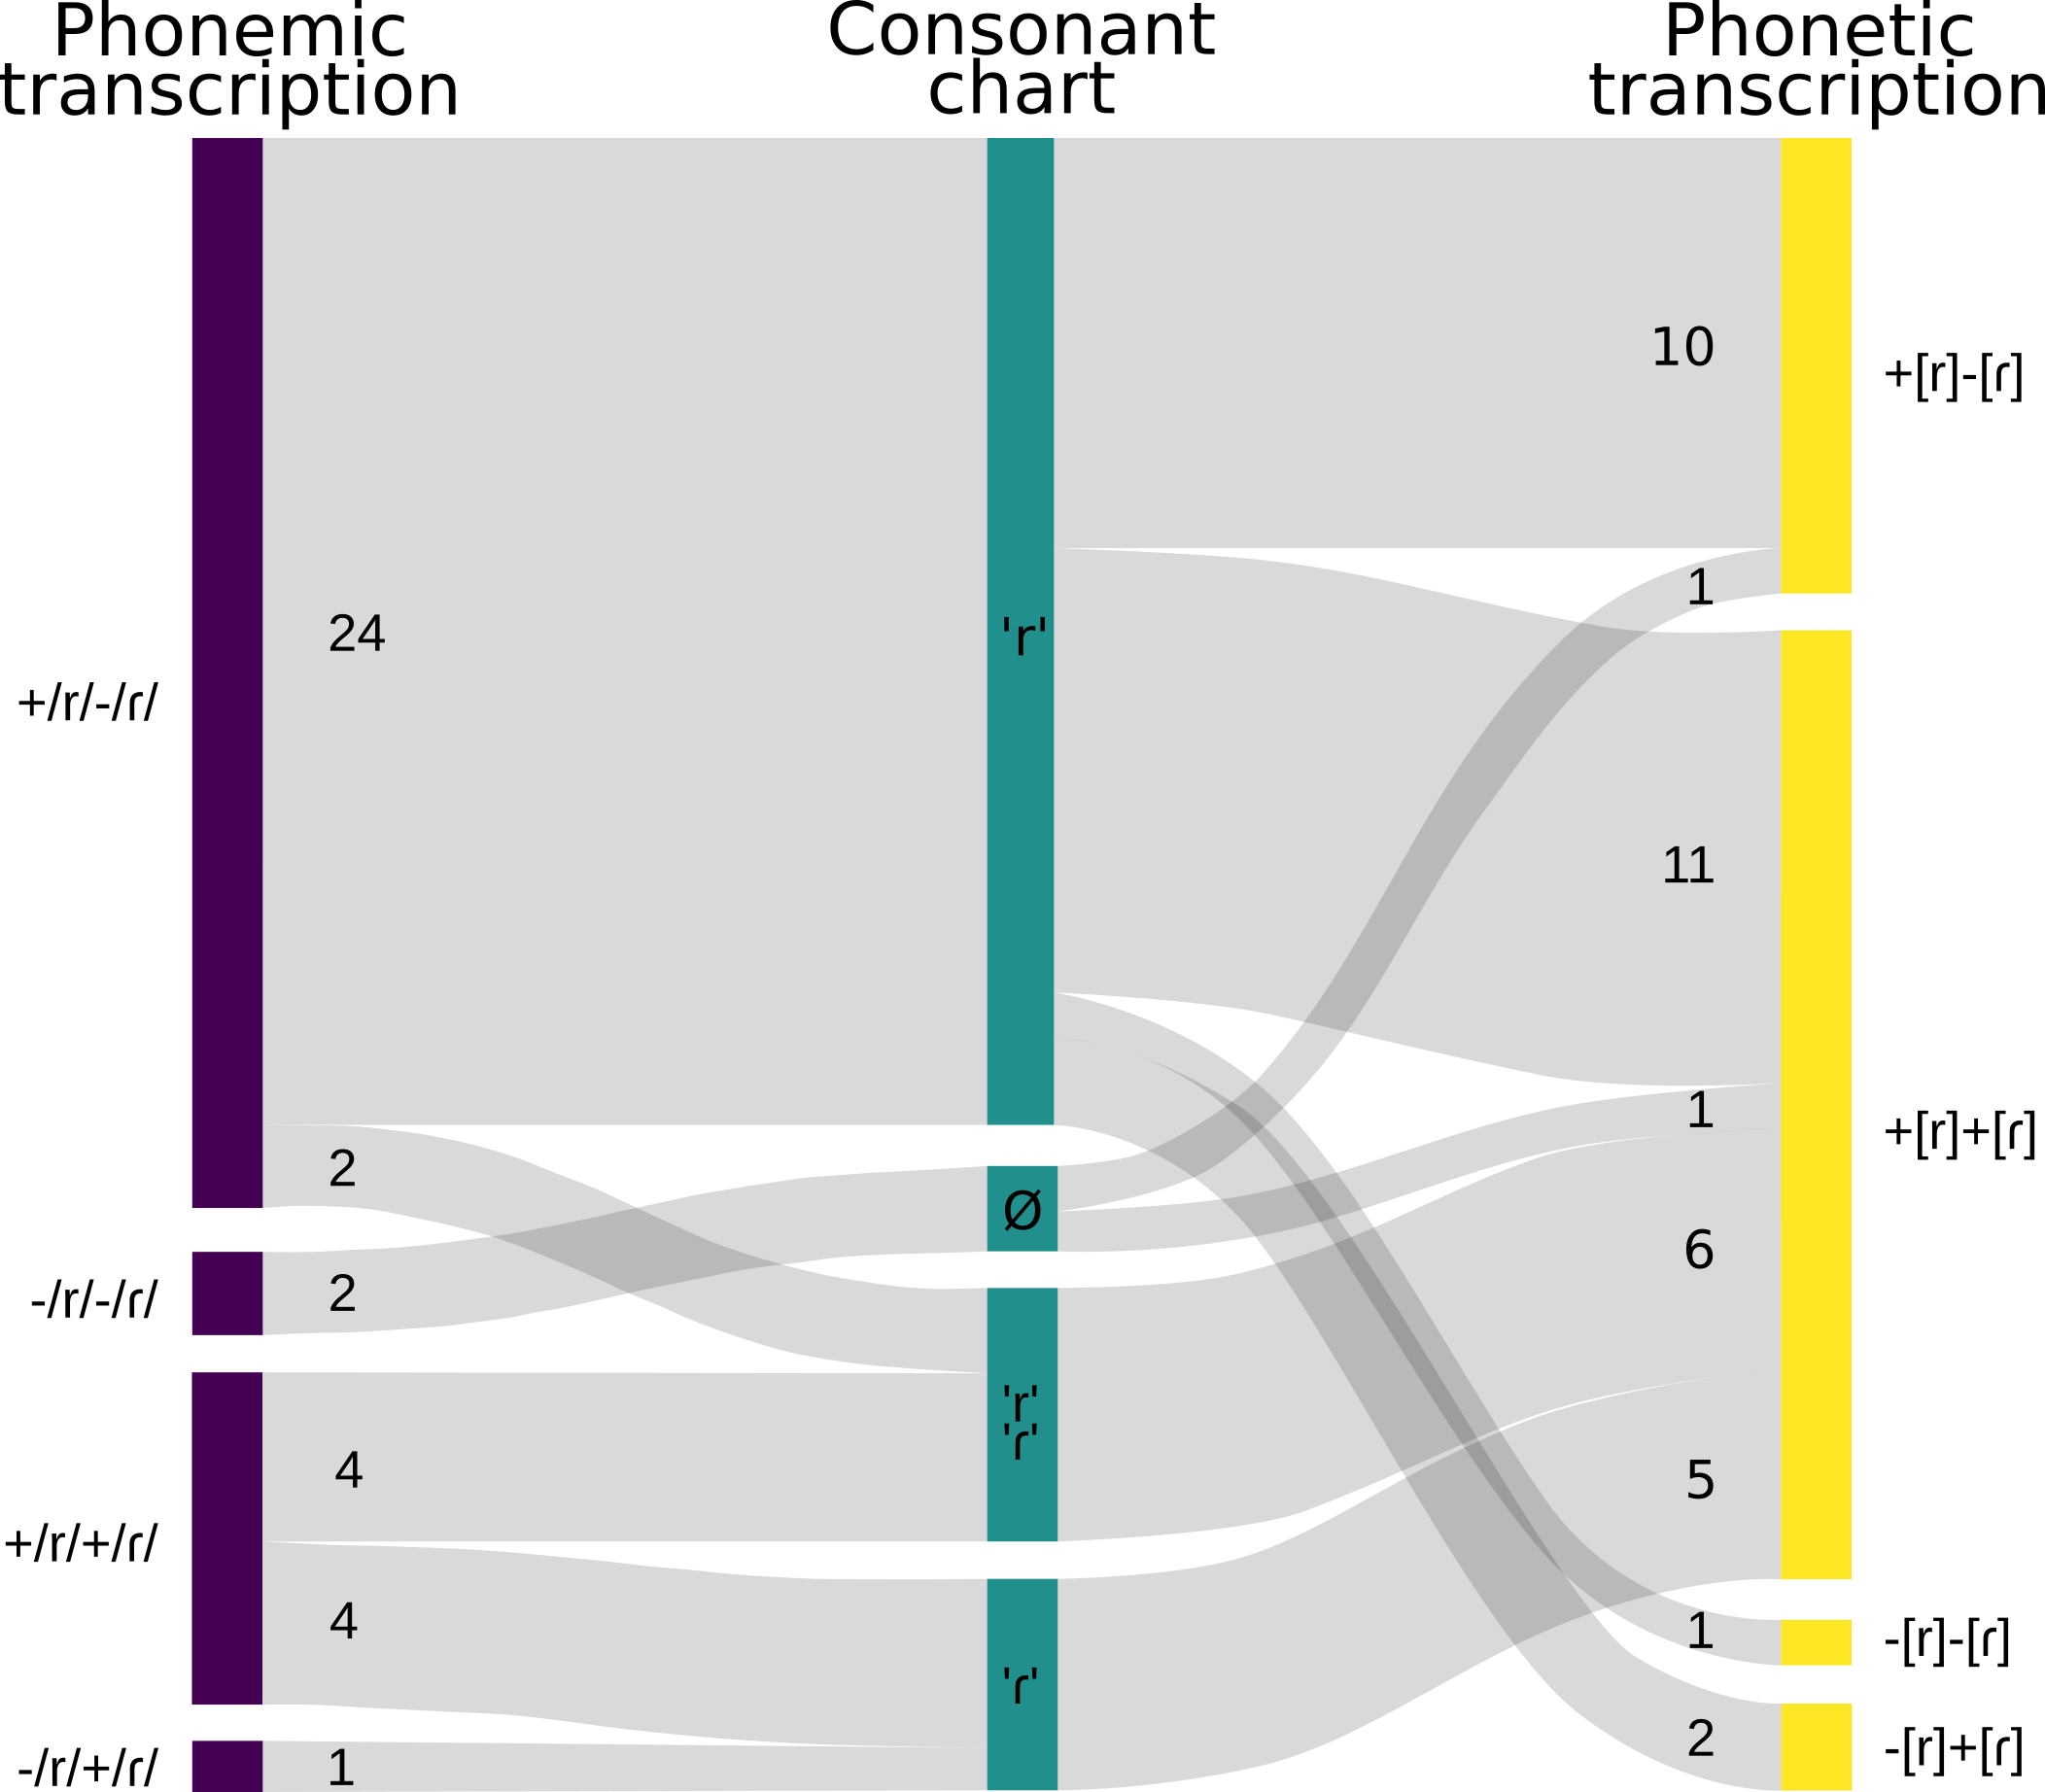
\includegraphics[width=0.75\linewidth]{jipa/images/sankey_phonemic_phonetic}
	\caption[Counts of illustrations with both phonemic and phonetic transcriptions when there is at least one \textit{r} in the illustration]{Counts of illustrations with both phonemic and phonetic transcriptions when there is at least one \textit{r} in the illustration, focusing on the phonemic transcription (left), the consonant chart (middle) and the phonetic transcription (right). The plus symbol (+) means the presence of \textit{r} in the narrative transcriptions and minus symbol (-) indicates its absence.}
	\label{fig:sankeyphonemicphonetic}
\end{figure}

We show a summary of these 37 illustrations in \autoref{fig:sankeyphonemicphonetic}. There are some interesting asymmetries between the use of \textit{r} in the phonetic and the phonemic transcriptions. For example, 24 illustrations contain an /r/ but do not contain an /ɾ/ in their phonemic transcription (left). All of these 24 illustrations include an \textit{r} in their consonant chart (left → middle). 10 of these 24 illustrations have a [r] but no [ɾ] in their phonetic transcription, 11 illustrations have a [r] and a [ɾ] in their phonetic transcription, one that in its phonetic transcription does not have any [r] or [ɾ], and two that have no [r] but only [ɾ] (middle → right). Also, there are two illustrations where both segments (trill and tap) are absent from the consonant chart (left → middle): in both cases, the phonemic transcriptions do not contain the segments, but the phonetic transcription for one illustration contains a [r] and for the other illustration it contains both segments [r] and [ɾ].\\

As shown in \autoref{fig:sankeyphonemicphonetic}, some authors do not always mention the \textit{r} in the consonant chart but do use the symbol in one of the transcriptions. In other cases, the use of \textit{r} in a phonemic transcription can be associated with a [r], with a [ɾ], with both, or even with none of these two segments. These results show that the presence of a [r] cannot be directly associated with a /r/ phoneme, in some cases the phonetic trill being associated with a /r/ but also with a /ɾ/, with both segments or even with none.

\newgeometry{inner=3.81cm,outer=3.81cm}

\begin{landscape}
\begin{longtable}{>{\raggedright\arraybackslash}m{4.5cm}cccc>{\centering\arraybackslash}m{2.5cm}>{\raggedright\arraybackslash}m{8cm}}
	%\resizebox{\textwidth}{!}{
	
%\begin{tabular}{>{\raggedright\arraybackslash}m{3.5cm}cccc>{\centering\arraybackslash}m{1.5cm}>{\raggedright\arraybackslash}m{3cm}}
	\\ \hline
	Title & [r] & /r/ & [ɾ] & /ɾ/ & Phonemic rhotic total & All phonetic segments \\
	\hline
	Afrikaans & 36 & 37 & 0 & 0 & 37 & 1 omission, 36 r \\
	\hline
	Amarasi & 2 & 5 & 3 & 0 & 5 & 3 ɾ, 2 r \\
	\hline
	\cellcolor{pink!40}Argentine Spanish & \cellcolor{pink!40}3 & \cellcolor{pink!40}3 & \cellcolor{pink!40}31 & \cellcolor{pink!40}31 & \cellcolor{pink!40}34 & \cellcolor{pink!40}31 ɾ, 3 r \\
	\hline
	Australian English & 0 & 11 & 3 & 0 & 11 & 11 ɹ, 3 ɾ as allophone of /t/ \\
	\hline
	\cellcolor{pink!40}Belarusian & \cellcolor{pink!40}16 & \cellcolor{pink!40}16 & \cellcolor{pink!40}0 & \cellcolor{pink!40}0 & \cellcolor{pink!40}16 & \cellcolor{pink!40}16 r \\
	\hline
	British English: Received Pronunciation & 0 & 11 & 0 & 0 & 11 & 11 ɹ \\
	\hline
	Brunei Malay & 3 & 19 & 12 & 0 & 19 & 12 ɾ, 3 ɹ, 1 omission, 3 r \\
	\hline
	Cagliari Sardinian & 23 & 27 & 16 & 0 & 27 & 16 ɾ (of which 12 are allophones of /t d/), 23 r \\
	\hline
	Castilian Spanish & 2 & 36 & 34 & 0 & 36 & 34 ɾ, 2 r \\
	\hline
	\cellcolor{gray!20}Central Arrernte & \cellcolor{gray!20}1 & \cellcolor{gray!20}0 & \cellcolor{gray!20}21 & \cellcolor{gray!20}22 & \cellcolor{gray!20}22 & \cellcolor{gray!20}21 ɾ, 1 r (we did not include ɻ) \\
	\hline
	Eastern Andalusian Spanish & 3 & 12 & 28 & 22 & 34 & 28 ɾ, 3 omissions, 3 r \\
	\hline
	Gayo & 8 & 26 & 18 & 0 & 26 & 18 ɾ, 8 r \\
	\hline
	\cellcolor{pink!40}Goizueta Basque & \cellcolor{pink!40}15 & \cellcolor{pink!40}15 & \cellcolor{pink!40}13 & \cellcolor{pink!40}13 & \cellcolor{pink!40}28 & \cellcolor{pink!40}13 ɾ, 15 r \\
	\hline
	Greek Thrace Xoraxane Romane & 8 & 18 & 11 & 2 & 20 & 11 ɾ, 1 omission, 8 r \\
	\hline
	\cellcolor{gray!20}Indonesian Bajau (East Lombok)
	& \cellcolor{gray!20}2 & \cellcolor{gray!20}1 & \cellcolor{gray!20}29 & \cellcolor{gray!20}40 & \cellcolor{gray!20}41 & \cellcolor{gray!20}39 ɾ, 2 r \\
	\hline
	Italian & 15 & 28 & 11 & 0 & 28 & 11 ɾ, 1 ɹ, 1 t̚, 15 r (there is one ɹɾ included in the count of taps here and there are 5 rː) \\
	\hline
	\cellcolor{gray!20}Itunyoso Trique & \cellcolor{gray!20}4 & \cellcolor{gray!20}2 & \cellcolor{gray!20}5 & \cellcolor{gray!20}8 & \cellcolor{gray!20}10 & \cellcolor{gray!20}5 ɾ, 1 ɽ, 4 r \\
	\hline
%\end{tabular}}
%\begin{tabular}{>{\raggedright\arraybackslash}m{3.5cm}cccc>{\centering\arraybackslash}m{1.5cm}>{\raggedright\arraybackslash}m{3cm}}
%\hline
	\cellcolor{pink!40}Kalabari-ljo & \cellcolor{pink!40}50 & \cellcolor{pink!40}50 & \cellcolor{pink!40}0 & \cellcolor{pink!40}0 & \cellcolor{pink!40}50 & \cellcolor{pink!40}50 r \\

	Kazakh & 6 & 15 & 9 & 0 & 15 & 9 ɾ, 6 r \\
	\hline
	Liverpool English & 3 & 10 & 1 & 0 & 11 & 1 ɾ, 7 ɹ, 3 r \\
	\hline
	\cellcolor{pink!40}Mavea & \cellcolor{pink!40}36 & \cellcolor{pink!40}36 & \cellcolor{pink!40}0 & \cellcolor{pink!40}0 & \cellcolor{pink!40}36 & \cellcolor{pink!40}36 r \\
	\hline
	\cellcolor{pink!40}Notes on the phonetics of Latvian & \cellcolor{pink!40}19 & \cellcolor{pink!40}19 & \cellcolor{pink!40}0 & \cellcolor{pink!40}0 & \cellcolor{pink!40}19 & \cellcolor{pink!40}19 r \\
	\hline
	\cellcolor{gray!20}Philippine English (Metro Manila acrolect) & \cellcolor{gray!20}1 & \cellcolor{gray!20}0 & \cellcolor{gray!20}0 & \cellcolor{gray!20}0 & \cellcolor{gray!20}30 & \cellcolor{gray!20}18 ɹ, 11 ɝ, 1 r \\
	\hline
	Russian & 17 & 20 & 3 & 0 & 20 & 3 ɾ, 17 r \\
	\hline
	Sasak, Meno-Mené dialect & 0 & 10 & 9 & 0 & 10 & 9 ɾ, 1 omission \\
	\hline
	Saterland Frisian & 9 & 23 & 2 & 0 & 23 & 2 ɾ (but allophone of /t/), 3 omissions, 1 ɹ, 10 vowels, 9 r \\
	\hline
	\cellcolor{gray!20}Seenku & \cellcolor{gray!20}1 & \cellcolor{gray!20}0 & \cellcolor{gray!20}3 & \cellcolor{gray!20}0 & \cellcolor{gray!20}4 & \cellcolor{gray!20}3 ɾ, 1 r \\
	\hline
	\cellcolor{gray!20}Standard Georgian & \cellcolor{gray!20}10 & \cellcolor{gray!20}9 & \cellcolor{gray!20}23 & \cellcolor{gray!20}30 & \cellcolor{gray!20}39 & \cellcolor{gray!20}23 ɾ, 4 tʂ, 1 ɚ, 1 omission, 10 r \\
	\hline
	Standard Malay (Brunei) & 6 & 28 & 22 & 0 & 28 & 22 ɾ, 6 r \\
	\hline
	\cellcolor{pink!40}Tamambo & \cellcolor{pink!40}19 & \cellcolor{pink!40}19 & \cellcolor{pink!40}0 & \cellcolor{pink!40}0 & \cellcolor{pink!40}19 & \cellcolor{pink!40}19 r \\
	\hline
	\cellcolor{pink!40}Tashlhiyt Berber & \cellcolor{pink!40}18 & \cellcolor{pink!40}18 & \cellcolor{pink!40}0 & \cellcolor{pink!40}0 & \cellcolor{pink!40}18 & \cellcolor{pink!40}18 r \\
	\hline
	\cellcolor{pink!40}Trapezountian Pontic Greek in Etoloakarnania & \cellcolor{pink!40}2 & \cellcolor{pink!40}2 & \cellcolor{pink!40}20 & \cellcolor{pink!40}20 & \cellcolor{pink!40}22 & \cellcolor{pink!40}20 ɾ, 2 r \\
	\hline
	The dialect of Venice & 23 & 38 & 15 & 0 & 38 & 15 ɾ, 23 r \\
	\hline
	The Flemish-Brabant dialect of Orsmaal-Gussenhoven & 21 & 32 & 8 & 0 & 32 & 8 ɾ (of which one is ɾɹ), 3 omissions, 21 r \\
	\hline
	\cellcolor{pink!40}'The North Wind and the Sun' in the Breton of the Isle of Groix & \cellcolor{pink!40}26 & \cellcolor{pink!40}26 & \cellcolor{pink!40}0 & \cellcolor{pink!40}0 & \cellcolor{pink!40}26 & \cellcolor{pink!40}26 r \\
	\hline
	\cellcolor{pink!40}Ukrainian & \cellcolor{pink!40}21 & \cellcolor{pink!40}21 & \cellcolor{pink!40}0 & \cellcolor{pink!40}0 & \cellcolor{pink!40}21 & \cellcolor{pink!40}21 r \\
	\hline
	Zurich German & 19 & 21 & 0 & 0 & 21 & 2 ʁ, 19 r \\
	\hline
%\end{tabular}

%^}
	\caption[Comparison of counts of \textit{r} and \textit{ɾ} in illustrations with a phonetic and phonemic transcription]{Comparison of counts of \textit{r} and \textit{ɾ} in illustrations with a phonetic and phonemic transcription, with all the possible phonetic segments that can be associated with a phonemic rhotic segment (including instances where there is a rhotic in the phonemic transcription but no equivalent rhotic in the phonetic transcription) or that are \textit{r}-like segment (allophones of plosives). Unshaded rows correspond to illustrations where [r] is less frequent than /r/, gray rows correspond to illustrations where [r] is more frequent than /r/, and red lines correspond to illustrations where [r] is as frequent as /r/.}
	\label{tab:tablecompaphonophone}
\end{longtable}
\end{landscape}

\restoregeometry

We use the varieties of English as an example of how the use of the symbol \textit{r} instead of the symbol \textit{ɹ} for the alveolar approximant is driven by simplicity of use and not by phonetic or phonological reasons. This is clearly the case for Australian English and British English Received Pronunciation, where \textit{r} is found in the phonemic transcription while [ɹ] is the main allophone found in the phonetic transcription. Things are more complicated for Liverpool English, where [r], [ɾ] and [ɹ] are used in the phonetic transcription while the author only mentions [ɾ] and [ɹ] as allophones, leading to difficulties in interpreting the symbol \textit{r} since it is not specified in the illustration as a possible allophone of /r/. \\

The use of the symbol \textit{r} is not necessarily transparent in phonetic transcriptions. The symbol \textit{r} is found for Zurich German but its interpretation is made difficult by the fact that while /r/ may have alveolar and uvular allophones, [r] is not specified as one of them. It is therefore not possible to say with certainty which allophone has been represented. \\

The use of \textit{r} does not necessarily imply the occurrence of [r] in phonetic transcriptions. The Sasak, Meno–Mené dialect illustration uses the symbol \textit{r} for the phoneme in the phonemic transcription, but the symbol is absent from the phonetic transcription. The authors do specify that ‘/r/ is sometimes produced as an alveolar tap’ \parencite[97]{archangeliSasakMenoMeneDialect2020} while an actual trilled realization occurs in word initial and word final positions. All occurrences of /r/ in the transcription appear in intervocalic positions and are realized as [ɾ], with one occurrence of /r/ in a pre–nasal context being omitted. [ɾ] seems to be a common realization of /r/ when the latter has more than one allophone in the phonetic transcription.\\

In \autoref{tab:tablecompaphonophone}, the non–colored (i.e., white background) rows represent the illustrations where the number of \textit{r} tokens is lower in the phonetic transcription than in the phonemic one. The last column indicates how the segments are realized and hence highlights the variation in the realizations of the rhotics that the authors reported. The grayed rows in \autoref{tab:tablecompaphonophone} highlight the cases where in there are more \textit{r} in the phonetic transcription than in the phonemic one: except for Itunyoso Trique (where there is a difference of two more occurrences of [r]), for the rest of the illustrations the difference consists of one more [r].\\

Finally, it is important to highlight the red rows in \autoref{tab:tablecompaphonophone} (11 illustrations) which denote when the same number of \textit{r} tokens is present in both transcriptions. This can be interpreted either as there being no explicitly reported variation among rhotics in these illustrations, or that all the trills in the phonemic transcription are realized as phonetic trills. In three of these cases, there is a contrast between /ɾ/ and /r/, and in eight cases (including the three cases aforementioned), the transcription is said to be ‘narrow’, ‘semi–narrow’ or ‘detailed’, supporting our second hypothesis that /r/ are realized as [r]. For example, in Kalabari–Ilo, there are 50 tokens of /r/ in the phonemic transcription, realized as 50 tokens of [r] in the narrow transcription also provided. As allophones other than the trill are mentioned, we infer that all tokens of /r/ are trilled.

\paragraph{Illustrations with phonetic transcriptions only}

\begin{figure}
	\centering
	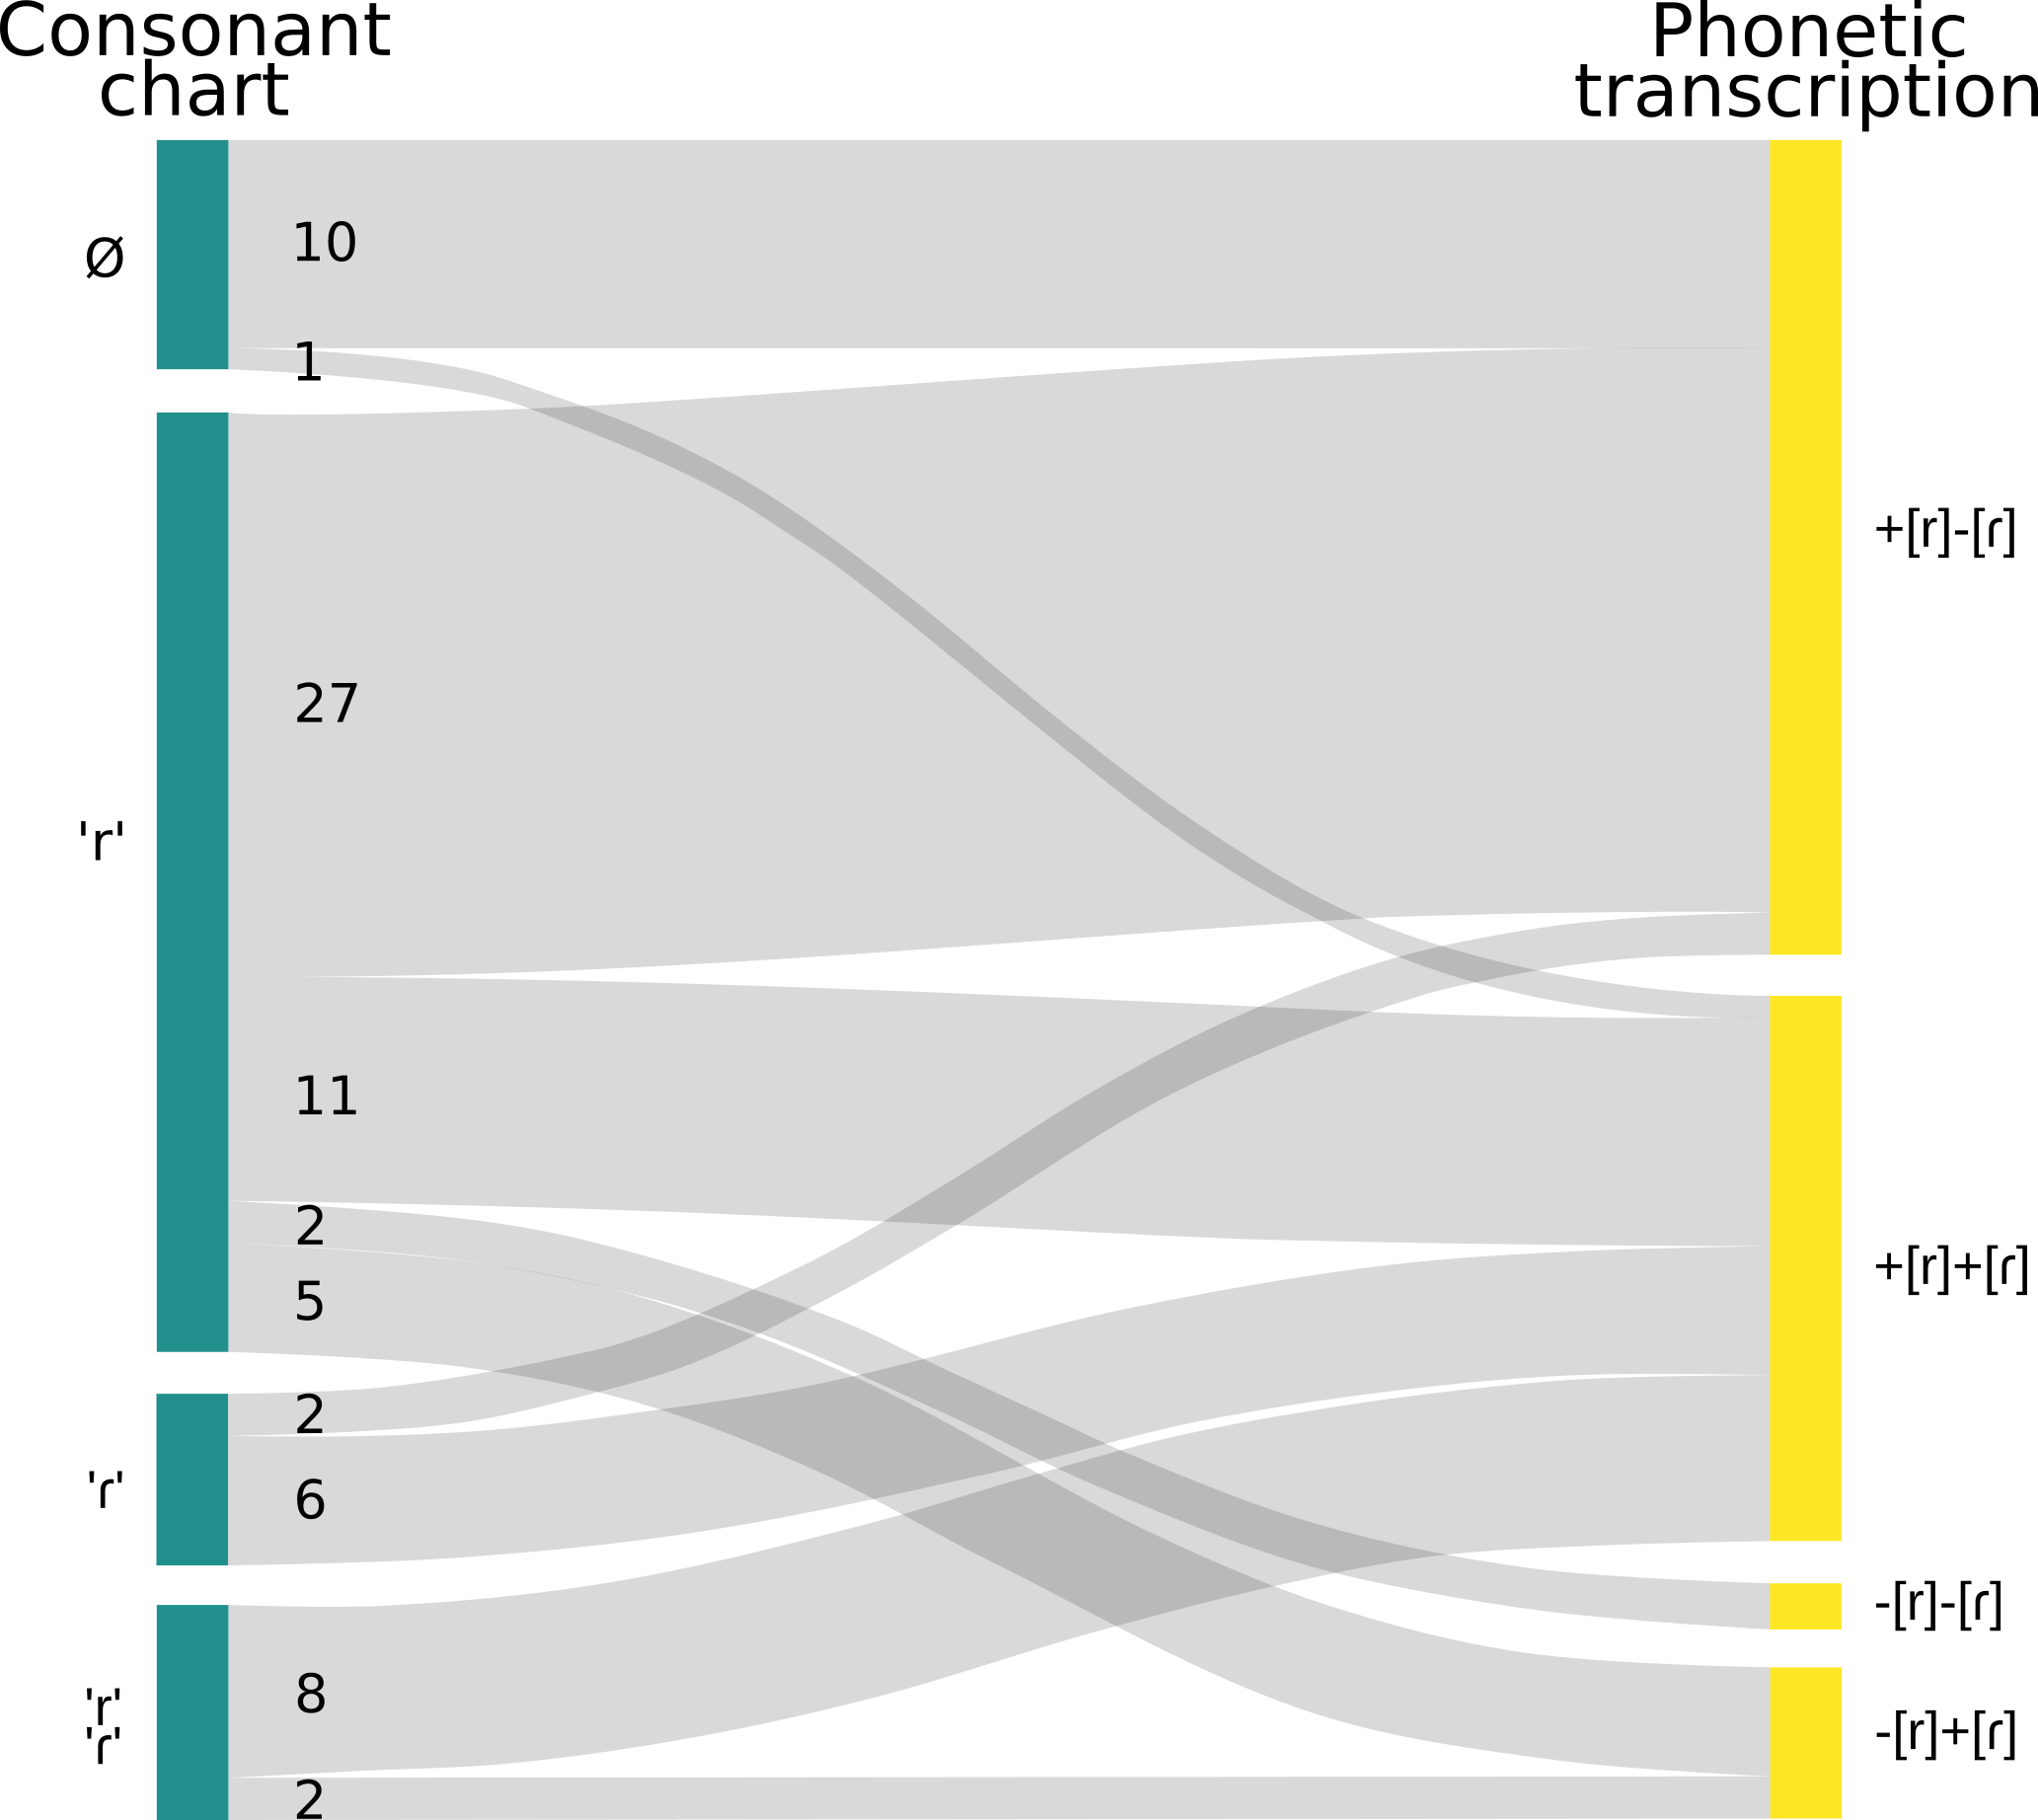
\includegraphics[width=0.75\linewidth]{jipa/images/sankey_phonetic}
	\caption[Counts of illustrations with a phonetic transcription only, which include at least one \textit{r} in the illustration]{Counts of illustrations with a phonetic transcription only, which include at least one \textit{r} in the illustration, focusing on the consonant chart (left) or on the phonetic transcription (right). The absence of \textit{r} in the consonant chart does not obligatorily imply that there will not be any [r] in the phonetic transcription, nor does the presence of \textit{r} obligatorily imply the presence of [r] in the phonetic transcription.}
	\label{fig:sankeyphonetic}
\end{figure}

Illustrations containing only an \textit{r} in their consonant chart have different types of possible production (\autoref{fig:sankeyphonetic}). We found illustrations where only [r] is present in the transcription (27 illustrations). In this first case, based on the author's transcription, we can consider that speakers are trilling for all the instances of their ‘r’. The second case corresponds to cases where there both [ɾ] and [r] are present (11 illustrations), both phones expected to be allophones of a /r/. The third case corresponds to the few illustrations which contain only [ɾ] in their transcription when a r was presented in the chart (five illustrations), and we finally find two illustrations where there is neither [r] nor [ɾ] in the transcription although the segment was present in the consonant table. Regarding the 10 illustrations where both  \textit{r} and \textit{ɾ} are present in the consonant chart, there is no [r] in the transcription for two of them while both phones [r] and  [ɾ] are found for the other eight.

\paragraph{Illustrations with a phonemic transcription only}

\begin{figure}
	\centering
	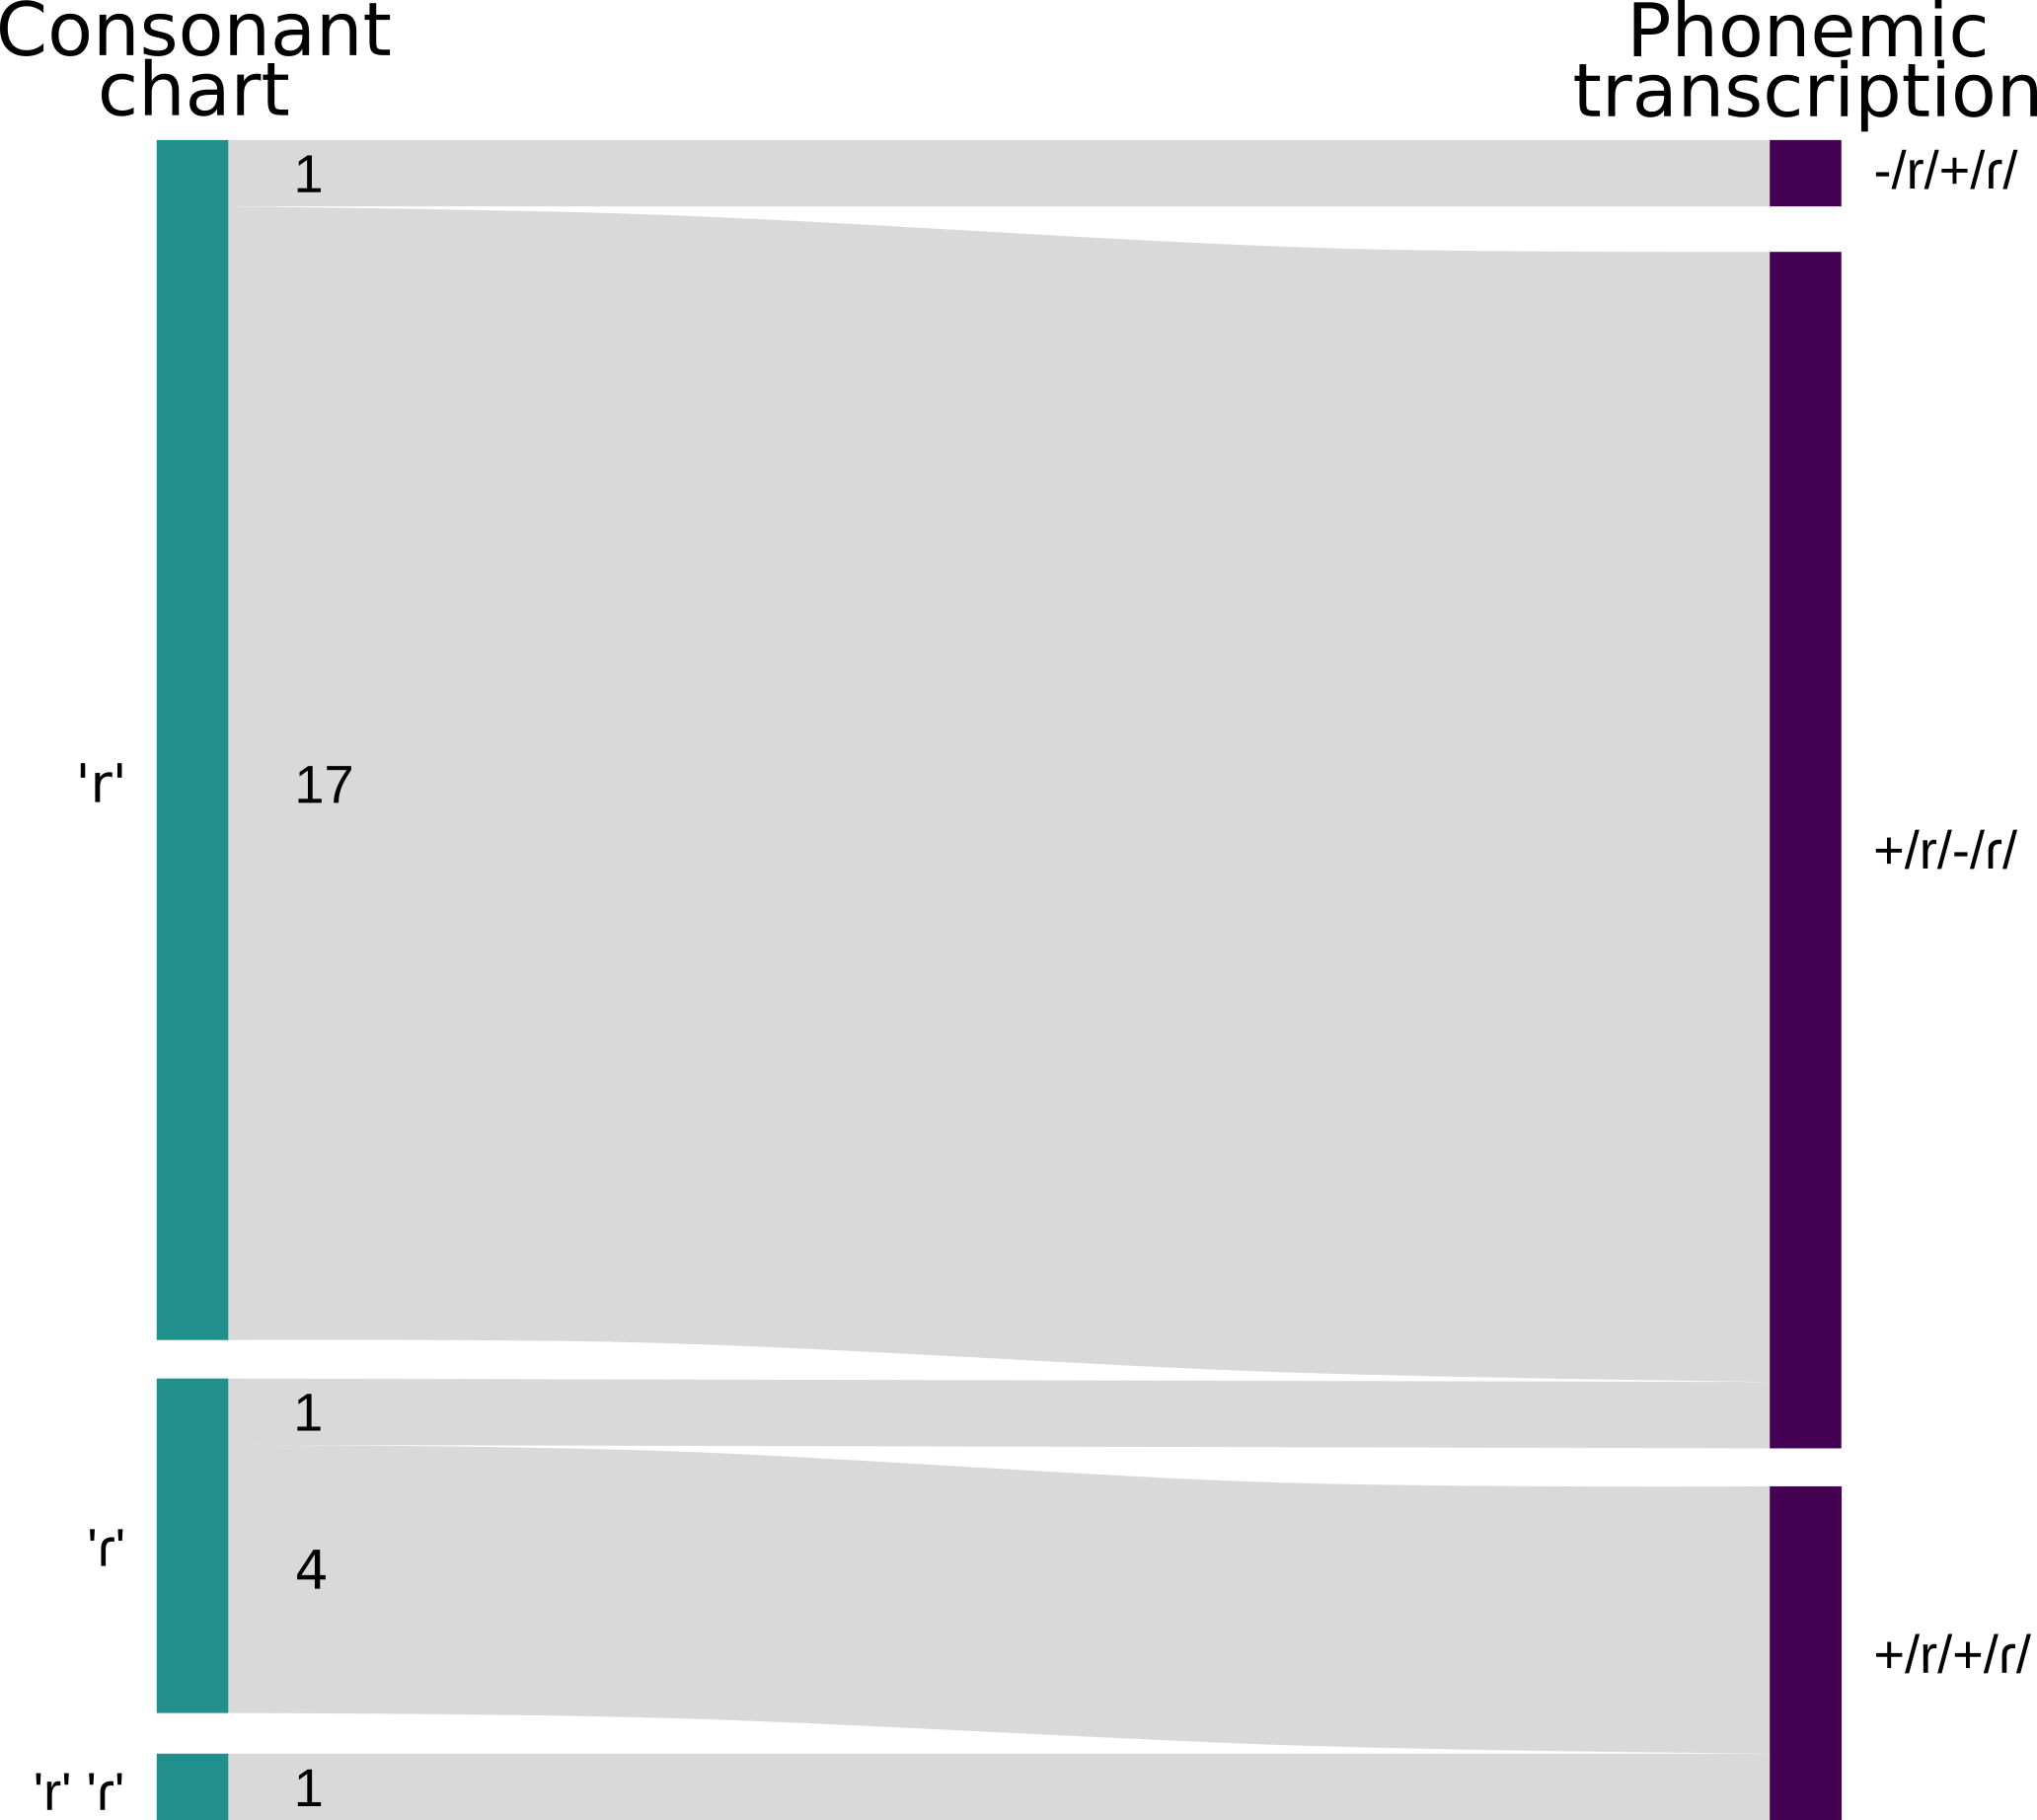
\includegraphics[width=0.75\linewidth]{jipa/images/sankey_phonemic}
	\caption[Counts of illustrations with a phonemic transcription only, which include at least one r in the illustration]{Counts of illustrations with a phonemic transcription only, which include at least one r in the illustration, focusing on the consonant chart (left) or on the phonemic transcription (right).}
	\label{fig:sankeyphonemic}
\end{figure}

Finally, it is important to also take into account the illustrations that are grouped in our third category, where we find only a phonemic transcription (\autoref{fig:sankeyphonemic}). Although their transcriptions refer to a level more abstract from the phonetic reality of the speaker’s production, one can still see differences between what is expected from the consonant chart and the symbols that are present in the transcription. In all the illustrations of this category except one, there is at least one /r/ in the phonemic transcription. In the remaining illustration, /r/ is absent from the phonemic transcription while /ɾ/ is present, in contrast with the consonant chart where there is only \textit{r} and not \textit{ɾ}.

\subsubsection{‘\textit{r}–like’ sound frequencies}

We then looked at the full transcriptions of the illustrations where there was at least one \textit{r}, in order to get at a first approximation of their frequency while taking all rhotic segments (i.e., all allophones of a rhotic phoneme) into account. Since the total number of segments and the number of rhotics differs across the illustrations, it is important to consider these in order to be able to meaningfully compare the frequency of \textit{r} among them.

\paragraph{Overall rhoticity}

The overall rhoticity, defined as freq$_\textrm{rhot}$ = n$_\textrm{ʀ}$ / n$_\textrm{seg}$, was computed based on all the possible segments that could be considered as rhotics in the transcription. Critical analysis of ambiguous segments (like the \textit{ɾ} which can be and allophone of a plosive, or \textit{ʁ} that can behave like a fricative but not like a rhotic) was done on the basis of the full illustration, so as to only select those segments that can be considered rhotics. For languages with two or more contrastive rhotics, this measure conflates all rhotic phonemes — it does not contain information on the relative frequencies of each rhotic phoneme individually.\\

\begin{figure}
	\centering
	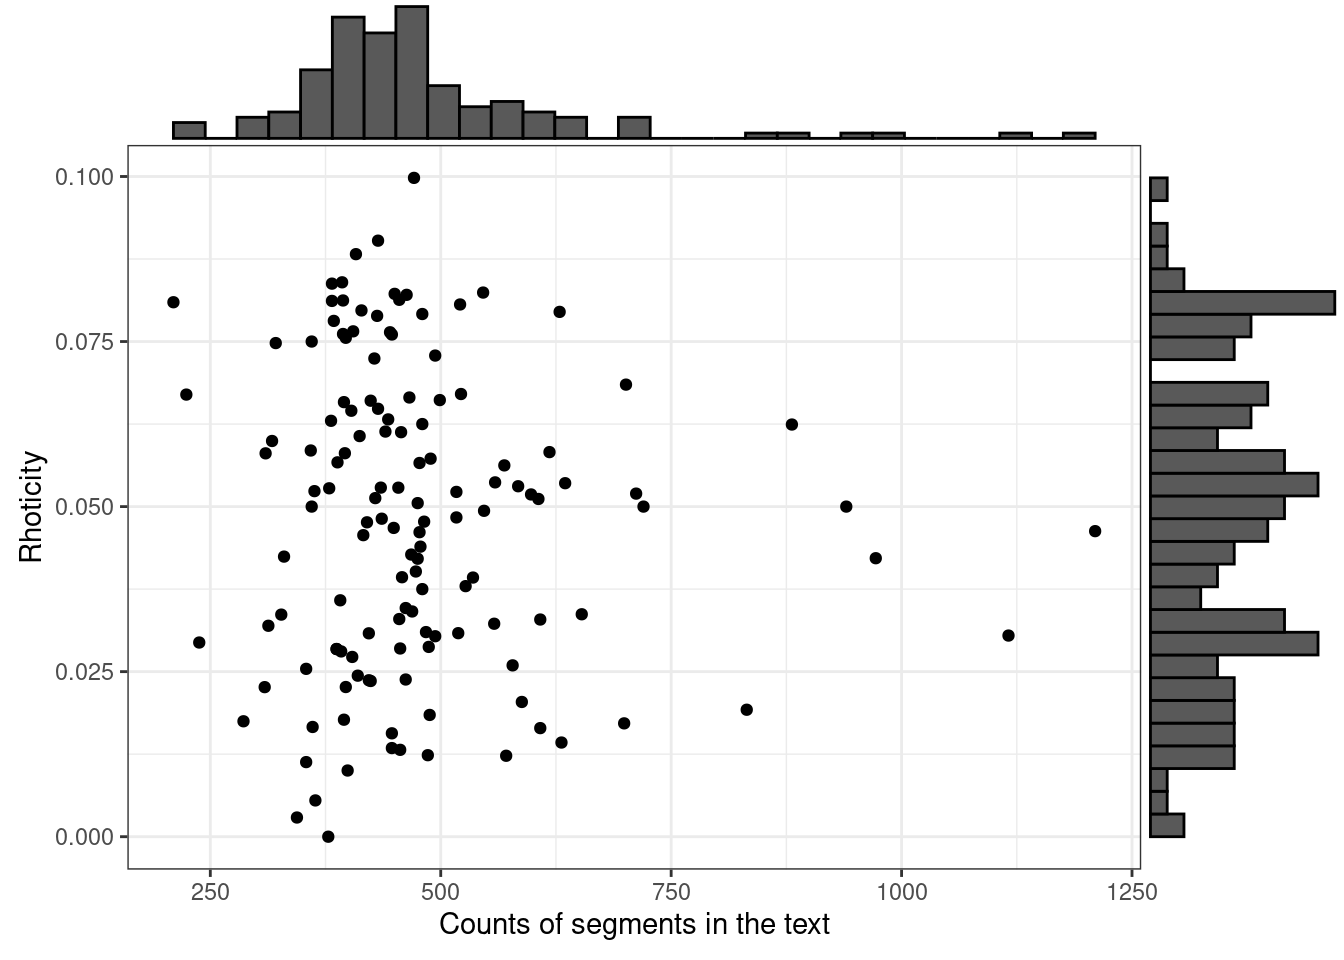
\includegraphics[width=0.75\linewidth]{jipa/images/rhoticy_freq}
	\caption[Rhoticity for the 135 transcriptions as a function of the number of segments in the written transcription]{Rhoticity for the 135 transcriptions on the vertical axis (1 illustration does not have any transcription and was removed) as a function of the number of segments in the written transcription on the horizontal axis.}
	\label{fig:rhoticyfreq}
\end{figure}

Unsurprisingly, \autoref{fig:rhoticyfreq} illustrates that not all transcriptions have the same length (minimum 210, mean 477.5, median 449, sd 148.5, IQR 122.5 and maximum 1210 segments). By dividing by the number of segments we control for text length in order to have a normalized estimate of rhoticity. There is variation in the rhoticity, freq$_\textrm{rhot}$ (minimum 0.0, mean 0.048, median 0.05, standard deviation sd 0.023, interquartile range IQR 0.035, and maximum 0.1). Figure 9 shows that it is not because a transcription contains a lot of segments that its overall rhotic frequency is high. For example, the transcription of the illustration of Shipibo \parencite{valenzuelaShipibo2001} contains 1116 segments while its rhoticity is about 0.03, on the other side, the illustration of Standard Georgian \parencite{shostedStandardGeorgian2006} contains 432 segments but its rhoticity is about 0.09 (one of the highest). A rhoticity of 0.0 corresponds to cases where there was an \textit{r} in the illustration but there wasn’t any rhotic in the narrative, possibly due to its very low frequency. This measure of rhoticity can be compared with estimates of trill and tap frequencies reported below.

\paragraph{Trill frequency}

\begin{figure}
	\centering
	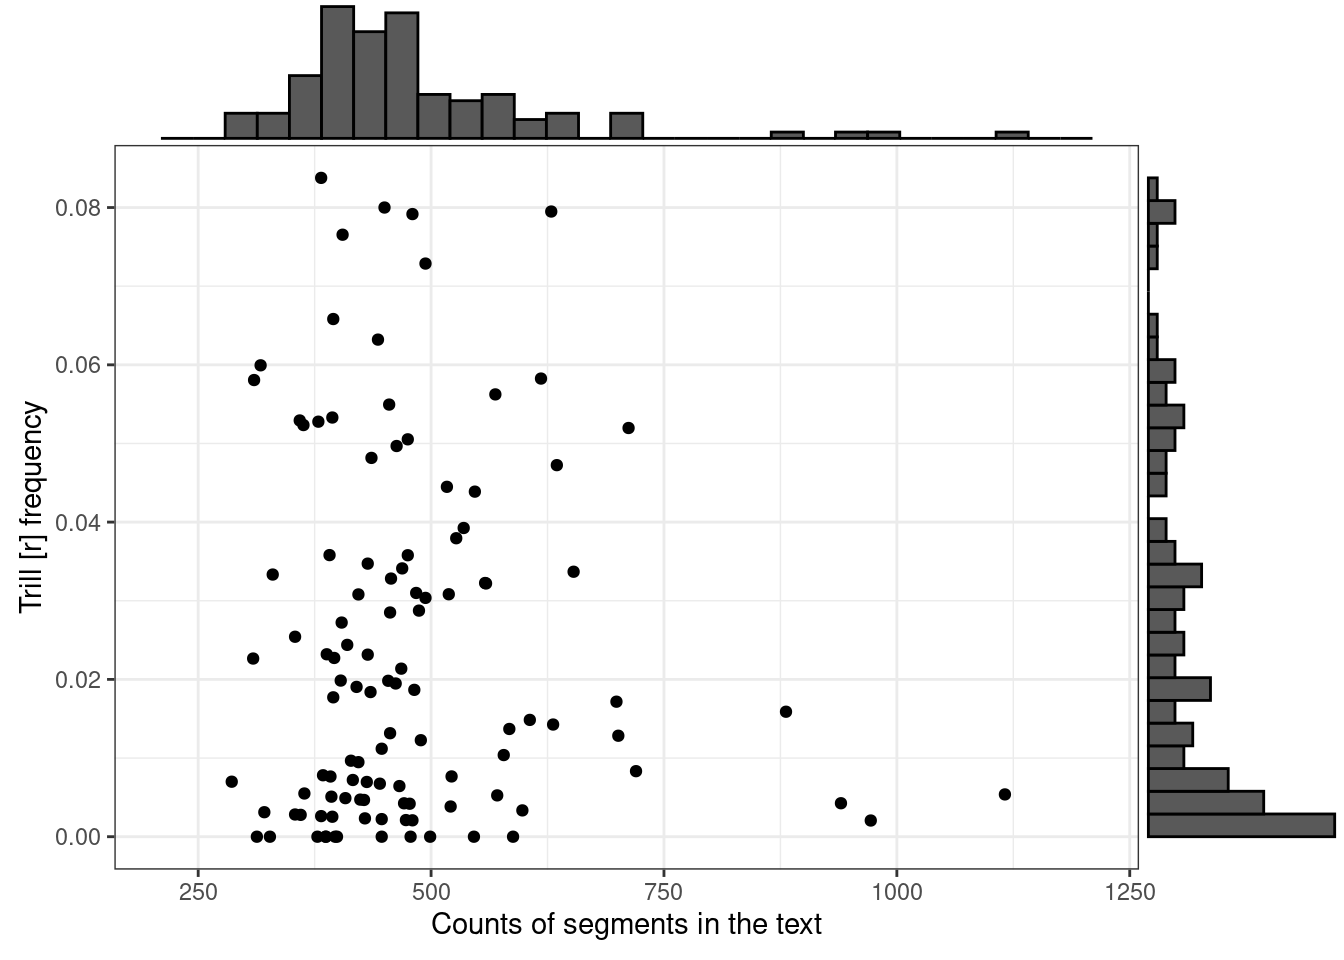
\includegraphics[width=0.75\linewidth]{jipa/images/trill_phonetic_freq}
	\caption[\textrm{[r]} frequency for the 111 transcriptions as a function of the number of segments in the written transcription]{[r] frequency (vertical axis) for the 111 transcriptions as a function of the number of segments in the written transcription (horizontal axis).}
	\label{fig:trillphoneticfreq}
\end{figure}

\autoref{fig:trillphoneticfreq} illustrates that the trill [r] frequency varies between a maximum of 0.084 (\textit{The dialect of Hasselt}) and a minimum of 0.0 (for 12 illustrations that do not contain [r] in their transcription), with a mean of 0.024, a median of 0.018 (both lower than for overall rhoticity), a standard deviation of 0.023, and an interquartile range of 0.031. A Wilcoxon test shows that the trill frequency is significantly lower than the mean of rhoticity 0.048 ($p<.0001$). This can be explained by the fact that in many cases the trill is not the only allophone used in the transcription to represent a rhotic segment (there are 43 illustrations where there is only one rhotic segment in the consonant chart, 28 where there are more than one rhotic segment in the consonant chart, and two illustrations where there is no rhotic segment in the consonant chart).


\begin{figure}
	\centering
	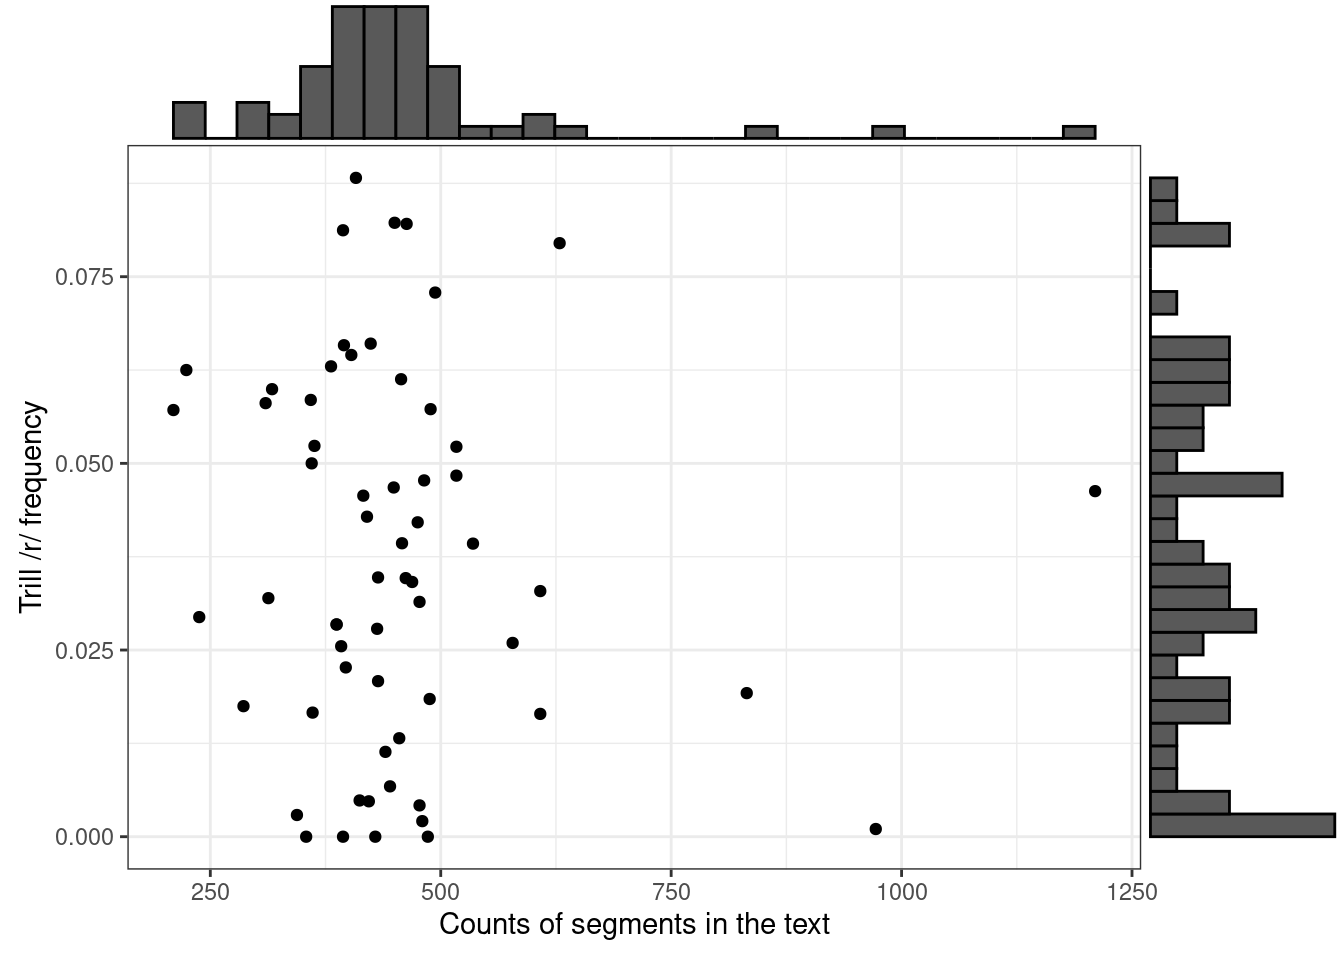
\includegraphics[width=0.75\linewidth]{jipa/images/trill_phonemic_freq}
	\caption[\textrm{/r/} frequency for the 61 transcriptions as a function of the number of segments in the written transcription]{/r/ frequency (vertical axis) for the 61 transcriptions as a function of the number of segments in the written transcription (horizontal axis).}
	\label{fig:trillphonemicfreq}
\end{figure}

\autoref{fig:trillphonemicfreq} illustrates that trill /r/ frequency varies between a maximum of 0.088 and a minimum of 0.0 (4 illustrations where there is no /r/ in the transcription of the narrative), with a mean of 0.037,  a median of 0.035 (both lower than for overall rhoticity), a standard deviation of 0.025, and an interquartile range of 0.04.\footnote{This maximum corresponds to Castilian Spanish, but it is important to mention that the broad transcription comes from Jones \& Dahl (1944: 16, mentioned by 	Martı́nez–Celdrán et al., 2003). The authors did not use the symbol \textit{ɾ} in opposition to \textit{r}, instead contrasted /r/ and /rr/ which are both counted in our analysis as instances of \textit{r}. This choice is consistent across all the illustrations that could have rr in their transcription (this contrast can also be found for the 2 more illustrations: Amharic and Cagliari Sardinian). Interestingly, Afrikaans is the illustration with the highest frequency of /r/ and the highest frequency of [r] if we exclude Castilian Spanish.} It can be seen that phonemic trill average frequency (0.037) is smaller than the average rhoticity (0.048), but higher than that of the phonetic trill (0.024), suggesting that the trills are more present in the phonemic transcriptions than in the phonetic ones. Figures 11 and 12 show that trill [r] and /r/ frequencies have different distributions when normalized by the total number of segments in the text. A Kruskal–Wallis test shows significant differences for frequency values of phonemic trill, phonetic trill and rhoticity ($H(2)=57.549,  p<.0001$), and a post hoc Dunn test shows that all the pairwise differences are statistically significantly different ($p<.01$).

\paragraph{Tap frequency}

We move now from the illustrations with at least one \textit{r}, to those with at least one \textit{ɾ} in either of the transcriptions or in the consonant chart. This new sample was composed of 95 illustrations with on average 488 segments per the transcription, and an average rhoticity of 0.048. A maximum of 2,410 segments was obtained for the illustration of Dàgáárè (Central).\\

\begin{figure}
	\centering
	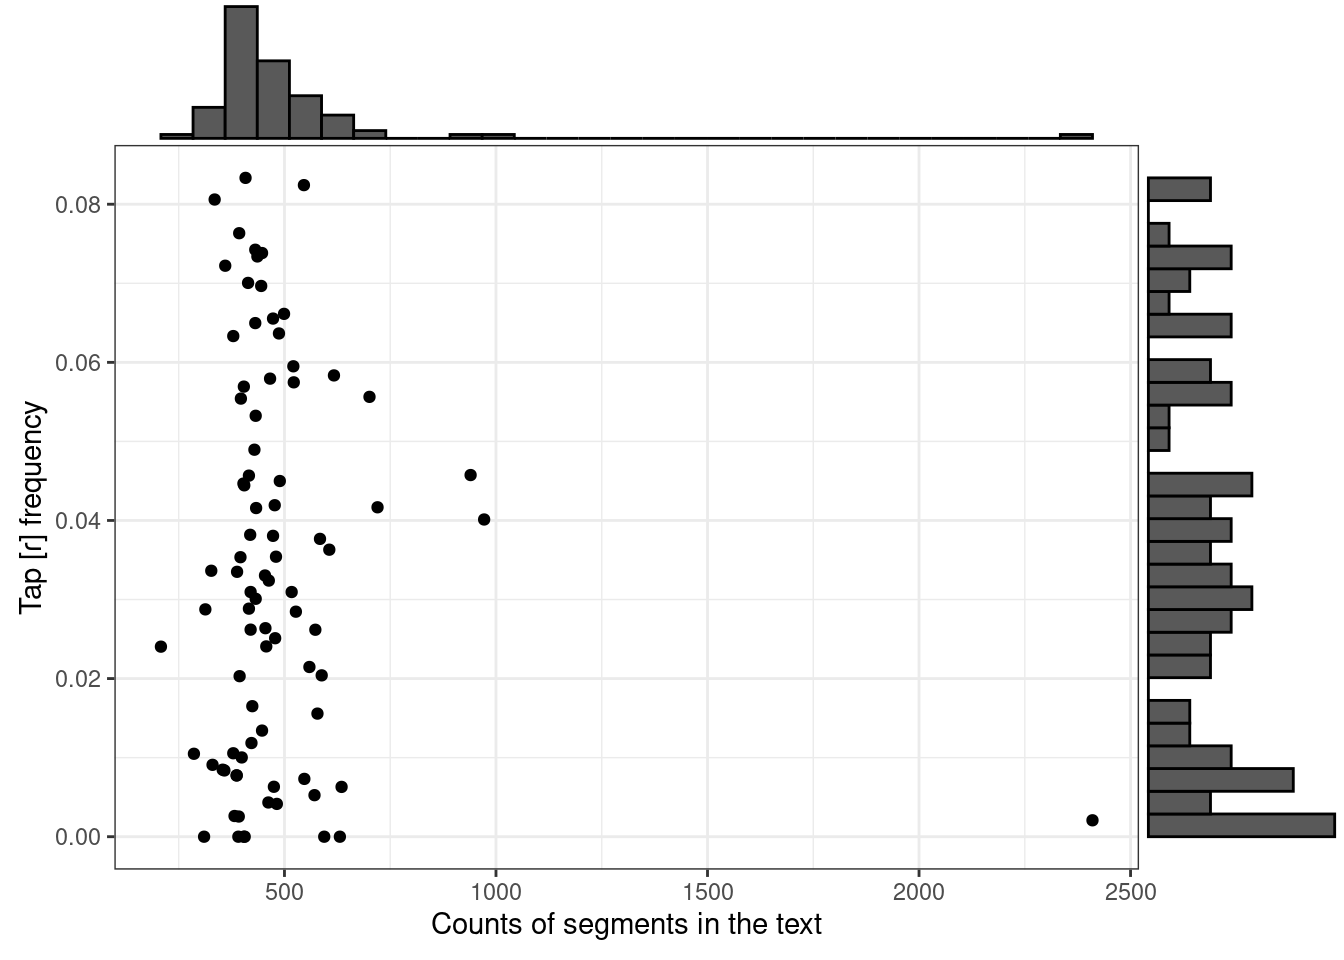
\includegraphics[width=0.75\linewidth]{jipa/images/tap_phonetic_freq}
	\caption[\textrm{[ɾ]} frequency for the 84 transcriptions as a function of the number of segments in the written transcription]{\textrm{[ɾ]} frequency (vertical axis) for the 84 transcriptions as a function of the number of segments in the written transcription (horizontal axis).}
	\label{fig:tapphoneticfreq}
\end{figure}

When looking at the taps in phonetic transcription (\autoref{fig:tapphoneticfreq}), the tap [ɾ] frequency varies between a maximum of 0.083 and a minimum of 0.0 (6 illustrations where there is no [ɾ] in the transcription of the narrative), with a mean of 0.034, a median of 0.032 (both lower than for overall rhoticity), a standard deviation of 0.024, and an interquartile range of 0.045. On the other hand, in phonemic transcription (Figure 13), the tap /ɾ/ frequency varies between a maximum of 0.07 and a minimum of 0.0 (22 illustrations where there is no /ɾ/ in the transcription of the narrative), with a mean of 0.02, and a median of 0.0 (both lower than for overall rhoticity), a standard deviation of 0.024, and an interquartile range of 0.039. The frequency of [ɾ] (0.034) is lower than the rhoticity average (0.048), but is higher than the frequency of /ɾ/. Phonetic taps are more frequent than phonemic taps. A Kruskal–Wallis test shows significant differences for frequency values of phonetic tap, phonemic tap and rhoticity ($H(2)=43.5, p<.0001$), and a post hoc Dunn test shows that all the pairwise differences are statistically significantly different ($p<.01$).

\begin{figure}
	\centering
	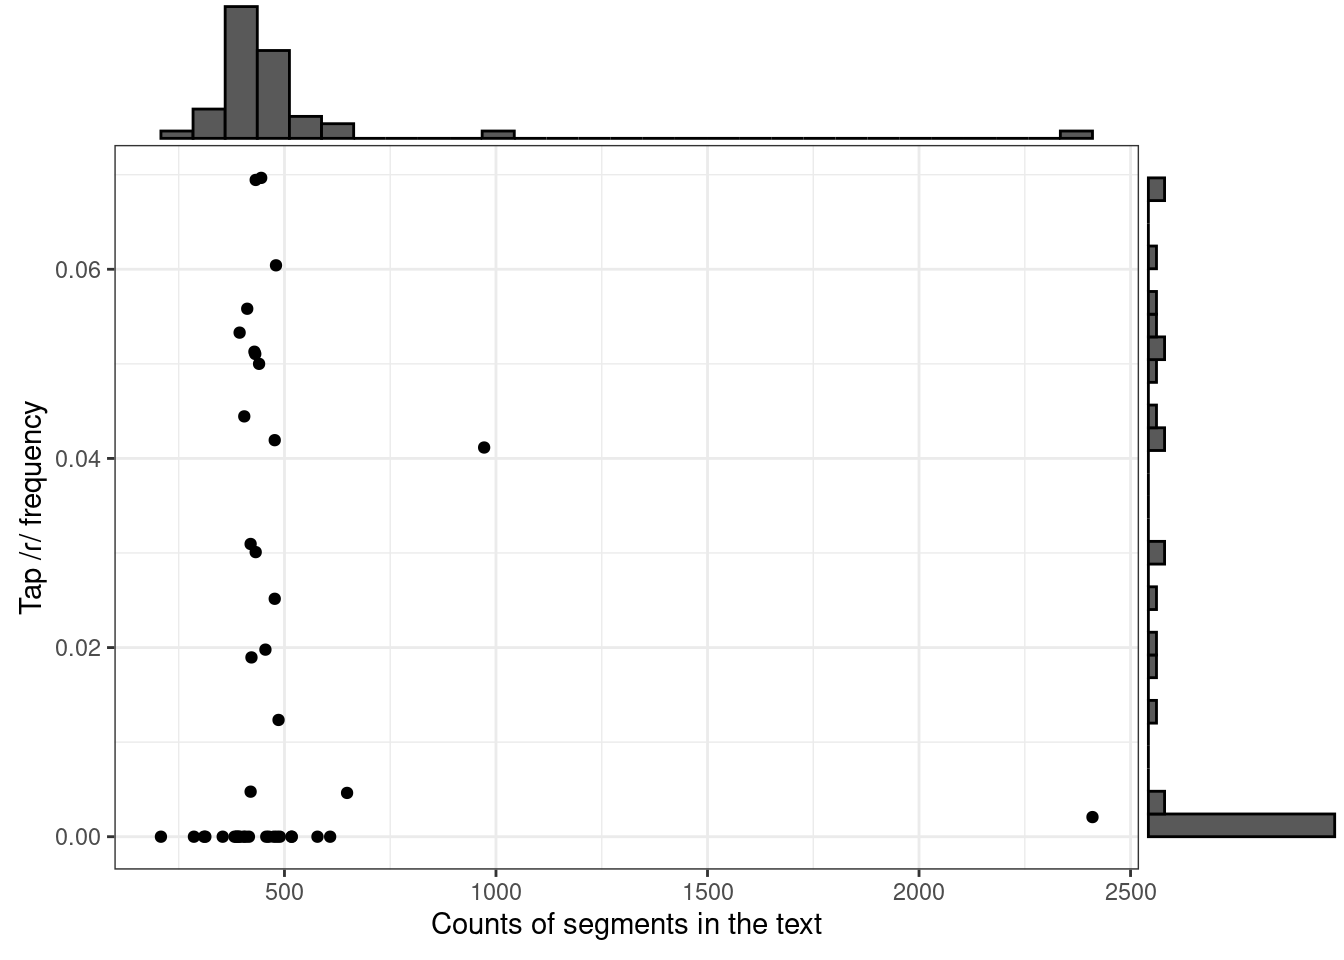
\includegraphics[width=0.75\linewidth]{jipa/images/tap_phonemic_freq}
	\caption[\textrm{/ɾ/} frequency for the 44 transcriptions as a function of the number of segments in the written transcription]{\textrm{/ɾ/} frequency (vertical axis) for the 44 transcriptions as a function of the number of segments in the written transcription (horizontal axis).}
	\label{fig:tapphonemicfreq}
\end{figure}

Finally, we compared the mean frequency of trills, taps and overall rhoticity: the Kruskal–Wallis test shows significant differences for frequency values ($H(4)=82.2, p<.0001$). A post hoc Dunn test showed that phonetic trills [r] frequency was not significantly different from the phonemic taps frequency /ɾ/, that phonemic trills /r/ frequency was not significantly different from the phonetic tap [ɾ] frequency, but that /r/ is more frequent than /ɾ/ ($p<.01$) and [r] is less frequent than [ɾ] ($p<.05$).\\

It can be seen that, compared to trills, taps are under–represented in phonemic transcriptions, but they are over–represented in phonetic transcriptions. The perceived abundance of trills is mainly due to their presence in the phonemic transcriptions, where the \textit{r} symbol encompasses, in fact, a multitude of possible phonetic realizations. One of these possible realizations is a tap, and even if phonetic trills are indeed present, they are less frequent than phonetic taps. These results do not explain why linguists choose certain graphic representations of the phonemes they describe, as the illustrations do not provide information on what makes a phonemic trill different from a phonemic tap. In some of the illustrations containing phonemic trills, we found both phonetic trills and taps, and similarly in some illustrations with phonemic taps, we found both phonetic taps and trills. An unequivocal analysis of a lect sound system based solely on its illustration may be unreachable in some cases due to linguist–specific graphemic conventions.

\section{Discussion and conclusions}

The \textit{Illustrations of the IPA} is an invaluable source of information for many types of studies in linguistics and the language sciences in general, as they tend to offer a standardized description of the sounds of the languages concerned. These articles stand on their own in providing the reader with the keys to understanding the conventions used in the phonetic and phonemic transcriptions. Importantly, they are also instrumental in linguistic studies – such as comparative studies – beyond their primary illustrative goal.\\

While, for some phonemes, transcription conventions are rich and accompanied by detailed descriptions of their different allophones, their context, and even, in some cases, by acoustic measurements, it appears that for rhotics such detailed information is often missing. This contributes to a lack of clarity in the literature concerning their characteristics and cross–linguistic frequency. While this situation seems to be improving in more recent illustrations, this lack of clarity was the reason for our study here. Rhotics are often represented through the symbol \textit{r}, but behind this seemingly simple choice there is a bewildering heterogeneity and complexity of realizations, as has been clearly shown for several languages (Spanish \parencites{blecuaVibrantesEspanolManifestaciones2002,bradleyRhoticVariationConstrast2012,henriksenAcousticAnalysisRhotic2015,vigilRhoticsTaosNew2018}, Dutch \parencite{sebregtsSociophoneticsPhonologyDutch2014}, Portuguese \parencite{rennickeVariationChangeRhotics2015}, English \parencites{stuart-smithDerhoticisationScottishEnglish2014,jauriberryRhotiquesRhoticiteEcosse2016}, Italian \parencite{romano2013preliminary}, Japanese \parencite{magnusonWhatSoundsKansai2008}, Persian \parencite{rafatSocioPhoneticInvestigationRhotics2010}).\\

This chapter quantifies, using a careful analysis of 213 \textit{Illustrations of the IPA} articles, the impression – shared by several linguists – that trills might be over–represented in the literature. We find that, although the phoneme /r/ is not rare (105 illustrations do have an /r/), [r] seems to become less and less frequent as one approaches the phonetic reality (here, as captured to various degrees by the phonetic transcriptions present in some of the illustrations). In other words, even with a transcription material as short as the North Wind and the Sun, we find consistent clues that the r trill symbol tends to be used as the default symbol for rhotics, echoing for instance Sebregts (2014) position:

\begin{displayquote}
~[...] the high cross–linguistic frequency of trill phonemes as reported in UPSID may not in fact be at odds with the low frequency of “actual trills” mentioned by \parencite{ladefogedLateralsTrills1977}, as long as the term “trill phoneme” in the sense of the UPSID is taken to mean a phoneme that is potentially realised as a trill, for which the number of actual trill realisations may be quite low. \parencite[157]{sebregtsSociophoneticsPhonologyDutch2014}
\end{displayquote}

As explained in this chapter, we consider that this ambiguity results from several factors that led the linguistic community to tolerate a blind spot which mirrors the difficulty of handling rhotics in general and trills in particular. We consequently suggest that clarifying the guidelines on rhotics would improve the gold standard against which \textit{Illustrations} is published as already proposed by \parencite[84]{whitleyRhoticRepresentationProblems2003} by ‘[a]dopt[ing] the macron for specifying a trill [ie. r̄], leaving plain \textbf{r} entirely free for its widely understood value of “any rhotic”’. Beyond this aspect, we would like to emphasize that the illustrations are also integrated ‘as they are’ in secondary sources such as phonological databases. There has indeed been a recent explosion in the availability and use of such databases \parencites{phoible,mortensenAlloVeraMultilingualAllophone2020}, and in their relevance to the exploration of large–scale typological and historical questions. Such databases usually compile data from different sources, among which we can find papers published in \textit{JIPA} (as, for example, in PHOIBLE and ALLOVERA). Irrespective of their intended nature (phonemic, allophonic or phonetic), they make use of the symbols proposed by transcription systems, and the symbols of the International Phonetic Alphabet (IPA) are omnipresent and currently almost universally used in linguistics. While they are arguably robust enough for large–scale studies concerning broad phonemic classes and their distribution across language families and geographical areas, our findings highlight that taking them at face value might not be sufficient for research aiming at uncovering subtle effects involving actual acoustic and/or articulatory features (such as those involving sound symbolism, the acoustic adaptation to the environment or weak effects of normal variation in the anatomy of the vocal tract). We hope that, in the near to medium future, this type of large–scale study will be able to better take into account the uncertainty concerning the actual sounds purportedly described by a symbol (and, of particular importance here, the trill), either through the availability of finer–grained data or of ways to probabilistically map a given symbol to a set of possible realizations in a given context. \\ 

Thus, our work should help better understand the current theories concerning the visual representation of languages, to judge their advantages, disadvantages and limits \parencites{whitleyRhoticRepresentationProblems2003,eslingPhoneticNotation2010,andersonCrosslinguisticDatabasePhonetic2018}.  \\    

To conclude, while we do not think there is a single ‘silver bullet’ that can solve all these issues, we suggest extra caution in the way phonetic symbols are interpreted, especially for older sources, and to contextualize them relative to the various transcription systems in use at the time and even relative to the reforms of the International Phonetic Association.